% Trabalho de Oficina de Planejamento e Governança Metropolitana
%
% Abaixo seguem orientações originais do modelo utilizado.
%
% Siga para o conteúdo do trabalho descendo até a linha 908.
%
% ==============================================================
%
% Modelo para monografia de final de curso, em conformidade
% com normas da ABNT implementadas pelo projeto abntex2.
%
% Este arquivo é fortemente baseado em exemplo distribuído no
% mesmo projeto. O projeto abntex2 pode ser acessado pela página
% http://abntex2.googlecode.com/
%
% Este arquivo pode ser rodado tanto com o pdflatex quanto com
% o lualatex.  Como contém referências bibliográficas a serem
% processadas pelo programa bibtex, este programa deve ser
% executado. Em resumo, a ordem de execução deve ser:
% rodar primeiro o pdflatex (ou o lualatex), depois o bibtex e,
% a seguir, o pdflatex (ou o lualatex ) novamente mais duas vezes,
% para assegurar que todas as referências bibliográficas e 
% citações estejam atualizadas.
%
% Para adaptar os textos para uso pessoal, usar os comandos
% imediatamente antes do \begin{document} (iniciando com o
% comando \titulo).  
%
% Este modelo está adaptado para monografias de final de curso
% em matemática da UFRJ, mas, com o uso das variáveis, pode ser
% usado para outros tipos de trabalho (mestrado, doutorado),
% outros cursos, universidades etc.  Caso a adaptação das
% variáveis não seja suficiente, pode-se alterar os comandos
% imprimircapa, imprimirfolhaderosto e imprimiraprovação, 
% fazendo as alterações necessárias.  Como os comandos definidos
% neste texto usam somente LaTeX, a sua adaptação deve ser 
% simples, bastando algum conhecimento de LaTeX.
%
% O restante do preâmbulo provavelmente  não necessitará ser
% alterado, a menos, eventualmente, das opções de chamada da
% classe abntex2, que estão definidas a seguir.
% 
\documentclass[ 
% -- opções da classe memoir que é a classe base da abntex2 --
% tamanho da fonte
12pt,
% capítulos começam em pág ímpar. Insere pág vazia, se preciso
openright,
% para imprimir uma página por folha ou visualização em video 
oneside,
% frente e verso. Margens das pag. ímpares diferem das pares.
%  twoside,
% tamanho do papel. 
a4paper,
% Caio - Ocultando bordas horríveis em hiperligações
hidelinks,
% -- opções da classe abntex2 --
% títulos de capítulos convertidos em letras maiúsculas
%  chapter=TITLE,
% títulos de seções convertidos em letras maiúsculas
%  section=TITLE,
% títulos de subseções convertidos em letras maiúsculas
%  subsection=TITLE,
% títulos de subsubseções convertidos em letras maiúsculas
%  subsubsection=TITLE,
% -- opções do pacote babel --
english,   % idioma adicional para hifenização
portuguese,   % o último idioma é o principal do documento
oldfontcommands,
]{abntex2}
%
% ==============================================================
%
% --------------------------------------------------------------
% Adicionando pacotes para recursos adicionais e defindo opções
% pertinentes
% --------------------------------------------------------------
%
% cabeçalho comum para uso com lualatex ou pdflatex
\usepackage{ifluatex}
% opções para uso com o lualatex
\ifluatex
\usepackage{fontspec}
\defaultfontfeatures{Ligatures=TeX}
% o fonte small caps é diferente no latin modern
\fontspec[SmallCapsFont={Latin Modern Roman Caps}]{Latin Modern Roman}
% pacotes da AMS 
\usepackage{amsmath,amsthm} 
% pacote para fonte específico para símbolos matemáticos
\usepackage{unicode-math}
\setmathfont{Latin Modern Math}
% latin modern tem simbolos de mathbb muito feios.
%  Trocar o fonte para estes simbolos.
\setmathfont[range=\mathbb]{Tex Gyre Pagella Math}
% opções para uso com o pdflatex
\else
\usepackage[utf8x]{inputenc}
\usepackage[T1]{fontenc}
\usepackage{lmodern}
\usepackage{etoolbox}
% pacotes da AMS 
\usepackage{amsmath,amssymb,amsthm} 
% Mapear caracteres especiais no PDF
\usepackage{cmap}
\fi

% pacotes usados tanto pelo lualatex quanto pelo pdflatex
\usepackage{lastpage}    % Usado pela Ficha catalográfica
\usepackage{indentfirst} % Indenta primeiro parágrafo 
\usepackage{color}       % Controle das cores
\usepackage{graphicx}    % Inclusão de gráficos
\usepackage{wrapfig}     % gráficos ao redor do texto
% pacote para ajustar os fontes em cada linha de forma a
% respeitar as margens
\usepackage{microtype}
% permite a gravação de texto em um arquivo indicado a partir
% deste arquivo.  Originalmente foi usado para criar o arquivo
% .bib com conteúdo de exemplo, evitando a edição de um arquivo
% .bib somente para a bibliografia
\usepackage{filecontents}

% Caio - diagramas
% http://www.texample.net/tikz/examples/smart-priority/
%\usepackage{smartdiagram}

% Caio - ladeando imagens
% https://tex.stackexchange.com/questions/57433/cannot-use-caption-under-minipage
\usepackage{caption}

% Caio - preciso de tabelas longas
% http://www.tex.ac.uk/FAQ-figurehere.html
\usepackage{longtable}

% Caio - quero alternar as cores das linhas da tabela
% https://tex.stackexchange.com/questions/107944/alternate-row-colors-in-longtable
\usepackage[table]{xcolor}
\definecolor{lightgray}{gray}{0.9}

% Caio - tentando melhorar o posicionamento das imagens
\usepackage{float}

% Caio - corrigindo espaçamento conforme http://tex.stackexchange.com/questions/5683/how-to-remove-top-and-bottom-whitespace-of-longtable
\setlength{\LTpre}{0pt}
\setlength{\LTpost}{0pt}

% Caio - preciso de plotagens
%\usepackage{pgfplots}
%\pgfplotsset{compat=1.8}

% Caio - quero usar letras nas listas do enumerate conforme https://tex.stackexchange.com/questions/2291/how-do-i-change-the-enumerate-list-format-to-use-letters-instead-of-the-defaul
\usepackage{enumitem}

% Caio - modo paisagem para tabelões
\usepackage{lscape}

% Caio - adicionando o pacote hyperref
\usepackage{hyperref}
% - e definindo metadados do PDF e comportamento dos links
\hypersetup{
	%pagebackref=true,
	pdftitle={Produto III}, 
	pdfauthor={Vários},
	pdfsubject={governança metropolitana},
	colorlinks=false,      		% false: boxed links; true: colored links
	linkcolor=blue,          	% color of internal links
	citecolor=blue,        		% color of links to bibliography
	filecolor=magenta,      	% color of file links
	urlcolor=blue,
	bookmarksdepth=4
}

% Caio - separação silábica
%\hyphenation{}

% Caio - citações mais poderosas
%\usepackage[autostyle]{csquotes}

%-----------------------------------------------------------
%-----------------------------------------------------------
% Caio - habilitar glossário
\usepackage{glossaries}
\makeglossaries

% \newglossaryentry{ex}{name={sample},description={an example}}
\newglossaryentry{rmc}{
	name={RMC},
	description={Região Metropolitana de Curitiba}
}

\newglossaryentry{comec}{
	name={COMEC},
	description={Coordenação da Região Metropolitana de Curitiba}
}

\newglossaryentry{ippuc}{
	name={IPPUC},
	description={Instituto de Pesquisa e Planejamento Urbano de Curitiba}
}

\newglossaryentry{fpics}{
	name={FPICs},
	description={Funções públicas de interesse comum}
}

\newglossaryentry{regic}{
	name={REGIC},
	description={Regiões de Influência das Cidades}
}

\newglossaryentry{rm}{
	name={RM},
	description={Região Metropolitana}
}

\newglossaryentry{rms}{
	name={rms},
	description={Regiões Metropolitanas}
}

\newglossaryentry{ipardes}{
	name={IPARDES},
	description={Instituto Paranaense de Desenvolvimento Econômico e Social}
}

\newglossaryentry{ibge}{
	name={IBGE},
	description={Instituto Brasileiro de Geografia e Estatística}
}

\newglossaryentry{rit}{
	name={RIT},
	description={Rede Integrada de Transporte}
}

\newglossaryentry{nuc}{
	name={NUC},
	description={Núcleo Urbano Central}
}

\newglossaryentry{cic}{
	name={CIC},
	description={Cidade Industrial de Curitiba}
}

\newglossaryentry{ciar}{
	name={CIAR},
	description={Centro Industrial de Araucária}
}

%-----------------------------------------------------------
%-----------------------------------------------------------
% Comandos para definir ambientes tipo teorema em português 
\newtheorem{meuteorema}{Teorema}[chapter]
\newtheorem{meuaxioma}{Axioma}[chapter]
\newtheorem{meucorolario}{Corolário}[chapter]
\newtheorem{meulema}{Lema}[chapter]
\newtheorem{minhaproposicao}{Proposição}[chapter]
\newtheorem{minhadefinicao}{Definição}[chapter]
\newtheorem{meuexemplo}{Exemplo}[chapter]
\newtheorem{minhaobservacao}{Observação}[chapter]
%-----------------------------------------------------------
%-----------------------------------------------------------
% Pacotes de citações
\usepackage[brazilian,hyperpageref]{backref}
\usepackage[alf]{abntex2cite}   % Citações padrão ABNT
%\usepackage[num]{abntex2cite}  % Citações numéricas
% --- 
% Configurações do pacote backref
% Usado sem a opção hyperpageref de backref
\renewcommand{\backrefpagesname}{Citado na(s) página(s):~}
% Texto padrão antes do número das páginas
\renewcommand{\backref}{}
% Define os textos da citação
\renewcommand*{\backrefalt}[4]{
	\ifcase #1 %
	Nenhuma citação no texto.%
	\or
	Citado na página #2.%
	\else
	Citado #1 vezes nas páginas #2.%
	\fi}%
% --- 
% --- 
% Espaço em branco no início do parágrafo
\setlength{\parindent}{1.3cm}
% Controle do espaçamento entre um parágrafo e outro:
\setlength{\parskip}{0.2cm}  % tente também \onelineskip
% ---
% compila o indice, se este for incluído no texto
\makeindex
%
% --------------------------------------------------------- 
% ---------------------------------------------------------
% Redefinindo o comando do abntex2 para gerar uma capa  
\renewcommand{\imprimircapa}{%
	\begin{capa}
		\begin{figure}
			\centering
			
\includegraphics[width=0.3\linewidth]{img/logotipo-ufabc-abaixo}
		\end{figure}	
		\begin{flushleft} 
			{\centering \Large \textsc{\imprimirinstituicao  \\
					\imprimircurso \\} }
		\end{flushleft}
		
		\vfill
		\begin{center}
			{\large \imprimirautor} \\
			\vspace*{0.5cm}
			{\Large \textit{\imprimirtitulo}}
		\end{center}
		
		\vfill
		\begin{center}
			{\large{\imprimirlocal \\ \imprimirano  }}
		\end{center}
		\vspace*{1cm} 
	\end{capa}
	
}

% ---------------------------------------------------------
% ---------------------------------------------------------
%
%
% ---------------------------------------------------------
% ---------------------------------------------------------
% Redefinindo o comando para gerar uma folha de rosto 
\renewcommand{\imprimirfolhaderosto}{%
	\begin{center}
		{\large \imprimirautor}
	\end{center}
	\vfill \vfill \vfill \vfill
	\begin{center}
		{\Large \textit{\imprimirtitulo}}
	\end{center}
	
	\vfill \vfill \vfill 
	\begin{flushright} 
		\parbox{0.5\linewidth}{
			\imprimirtipotrabalho\, relacionado ao 
			\imprimircurso\, da \imprimirsigla\, 
			entregue como parte do
			processo de graduação para a obtenção do 
			grau de \imprimirgrau.}
	\end{flushright} 
	
	\vfill 
	\begin{flushright} 
		\parbox{0.5\linewidth}{ \imprimirorientadorRotulo 
			\imprimirorientador\\ \imprimirttorientador}
	\end{flushright} 
	
	\ifdefvoid{\imprimircoorientador}{}{
		\begin{flushright} 
			\parbox{0.5\linewidth}{ \imprimircoorientadorRotulo 
				\imprimircoorientador\\ \imprimirttcoorientador}
		\end{flushright}
	}
	
	\vfill \vfill \vfill \vfill \vfill \vfill \vfill
	\begin{center}
		{\large{\imprimirlocal \\ \imprimirano}}
	\end{center}
	\vspace*{1cm} \newpage
}
% Final do comando para gerar uma folha de rosto 
% ---------------------------------------------------------
% ---------------------------------------------------------
%
%
% ---------------------------------------------------------
% ---------------------------------------------------------
% Definindo o comando para gerar uma folha de defesa 
\newcommand{\imprimirfolhadeaprovacao}{%
	\begin{center}
		{\large \imprimirautor}
	\end{center}
	\vfill \vfill \vfill \vfill
	\begin{center}
		{\Large \textit{\imprimirtitulo}}
	\end{center}
	
	\vfill \vfill \vfill \vfill \vfill \vfill
	\begin{flushright} 
		\parbox{0.5\linewidth}{
			%			\imprimirtipotrabalho\,apresentada ao 
			%			\imprimircurso\, da \imprimirsigla\, como requisito
			%			para a obtenção parcial do grau de \imprimirgrau.}
		}
	\end{flushright} 
	\vfill \vfill \vfill \vfill
	Aprovada em \data.
	
	\vfill \vfill \vfill \vfill
	
	\begin{center}
		\textbf{BANCA EXAMINADORA}
		
		\vfill\vfill\vfill
		\rule{10cm}{.1pt}\\
		{\imprimirexaminadorum} \\ {\imprimirttexaminadorum}
		
		\ifdefvoid{\imprimirexaminadordois}{}{
			\vfill\vfill
			\rule{10cm}{.1pt}\\
			\imprimirexaminadordois \\ \imprimirttexaminadordois }
		
		\ifdefvoid{\imprimirexaminadortres}{}{
			\vfill\vfill
			\rule{10cm}{.1pt}\\
			\imprimirexaminadortres \\ \imprimirttexaminadortres }
		
		\ifdefvoid{\imprimirexaminadorquatro}{}{
			\vfill\vfill
			\rule{10cm}{.1pt}\\
			\imprimirexaminadorquatro \\ \imprimirttexaminadorquatro }
	\end{center}
	
	\vfill \vfill 
	\begin{center}
		{\large{\imprimirlocal \\ \imprimirano}}
	\end{center}
	\vspace*{1cm}
	\newpage
}
% Final do comando para gerar uma folha de defesa 
% ---------------------------------------------------------
% --------------------------------------------------------
%
%
%
%
%
% ---------------------------------------------------------
% --------------------------------------------------------
% definindo variáveis adicionais 
\providecommand{\imprimirsigla}{}
\newcommand{\sigla}[1]{\renewcommand{\imprimirsigla}{#1}}
%
\providecommand{\imprimircurso}{}
\newcommand{\curso}[1]{\renewcommand{\imprimircurso}{#1}}
%
\providecommand{\imprimirano}{}
\newcommand{\ano}[1]{\renewcommand{\imprimirano}{#1}}
%
\providecommand{\imprimirgrau}{}
\newcommand{\grau}[1]{\renewcommand{\imprimirgrau}{#1}}
%
\providecommand{\imprimirexaminadorum}{}
\newcommand{\examinadorum}[1]{
	\renewcommand{\imprimirexaminadorum}{#1}}
%
\providecommand{\imprimirexaminadordois}{}
\newcommand{\examinadordois}[1]{
	\renewcommand{\imprimirexaminadordois}{#1}}
%
\providecommand{\imprimirexaminadortres}{}
\newcommand{\examinadortres}[1]{
	\renewcommand{\imprimirexaminadortres}{#1}}
%
\providecommand{\imprimirexaminadorquatro}{}
\newcommand{\examinadorquatro}[1]{
	\renewcommand{\imprimirexaminadorquatro}{#1}}
%
\providecommand{\imprimirttorientador}{}
\newcommand{\ttorientador}[1]{
	\renewcommand{\imprimirttorientador}{#1}} 
%
\providecommand{\imprimirttcoorientador}{}
\newcommand{\ttcoorientador}[1]{
	\renewcommand{\imprimirttcoorientador}{#1}}
%
\providecommand{\imprimirttexaminadorum}{}
\newcommand{\ttexaminadorum}[1]{
	\renewcommand{\imprimirttexaminadorum}{#1}}
%
\providecommand{\imprimirttexaminadordois}{}
\newcommand{\ttexaminadordois}[1]{\renewcommand{
		\imprimirttexaminadordois}{#1}}
%
\providecommand{\imprimirttexaminadortres}{}
\newcommand{\ttexaminadortres}[1]{
	\renewcommand{\imprimirttexaminadortres}{#1}}
%
\providecommand{\imprimirttexaminadorquatro}{}
\newcommand{\ttexaminadorquatro}[1]{
	\renewcommand{\imprimirttexaminadorquatro}{#1}}
% fim da definição de variáveis adicionais
% ---------------------------------------------------------
% ---------------------------------------------------------
%
% ---
% ---
% ---
% ---
% ---
% ---
% ---
% ---
% ---
% Informações de dados para CAPA, FOLHA DE ROSTO e FOLHA DE DEFESA
%
%----------------- Título e Dados do Autor -----------------
\titulo{Produto III: Caderno de Sustentação}
\autor{Caio César C. Ortega \and Gustavo Lopes Alcantara \and Mariana Lins Sartori \and Michele Almeida \and Victor Aranha Pereira
}
%

%----------Informações sobre a Instituição e curso -----------------
\instituicao{Universidade Federal do ABC \\
	Centro de Engenharia, Modelagem e Ciências Sociais Aplicadas}
%
\sigla{UFABC}
%
\curso{Bacharelado em Planejamento Territorial}
%\curso{Curso de Licenciatura em Matemática}
%\curso{Mestrado em Ensino de Matemática}
%\curso{Doutorado em Matemática}
%
\local{São Bernardo do Campo, SP}
%
%
% -------- Informações sobre o tipo de documento
\tipotrabalho{Relatório}
%\tipotrabalho{Monografia de final de curso}
%\tipotrabalho{Dissertação de mestrado}
%\tipotrabalho{Tese de doutorado}
%
\grau{BACHAREL em Planejamento Territorial}
%\grau{LICENCIADO em Matemática}
%\grau{MESTRE em Matemática}
%\grau{DOUTOR em Ciências}
%
\ano{2019}
\data{Dezembro de 2019} % data da aprovação
%
%------Nomes do Orientador, examinadores.  
\orientador{Prof. Dr. Jeroen Klink}
%\coorientador{Antonio da Silva} % opcional
\examinadorum{Profa. Dra. Silvana Zioni}
\examinadordois{Prof. Dr. Jeroen Klink}
%\examinadortres{Jeferson Leandro Garcia de Araújo}
%\examinadorquatro{Antonio da Silva}
%
%--------- Títulos do Orientador e examinadores ----
%\ttorientador{Bacharel em Física - UEFS}
%\ttcoorientador{Doutor em Matemática - UFRJ} 
%\ttexaminadorum{Doutor em Matemática - UFRJ}
%\ttexaminadordois{Doutor em Matemática - UFRJ}
%\ttexaminadortres{Doutor em Matemática - UFRJ}
%\ttexaminadorquatro{Doutor em Matemática - UFRJ}
%
% ---
% ---
\begin{document}
	
	% ---
	% Chamando o comando para imprimir a capa
	\imprimircapa
	% ---
	% ---
	% Chamando o comando para imprimir a folha de rosto
	%\imprimirfolhaderosto
	% ---
	% ---
	% Chamando o comando para imprimir a folha de aprovação
	%\imprimirfolhadeaprovacao
	% ---
	% ---
	% Dedicatória
	% ---
	%	\begin{dedicatoria}
	%  	 \vspace*{\fill}
	%  	 \centering
	%  	 \noindent
	%  	 \textit{ Este trabalho é dedicado a todos que, com entusiasmo,\\
	%  	 		sonham e lutam por XYZ no ABCDEFG\\
	%  			do XPTO.} \vspace*{\fill}
	%	\end{dedicatoria}
	%	
	%	
	%	\begin{agradecimentos}
	%	Orientação do modelo: insira aqui um parágrafo
	%	\end{agradecimentos}
	%	
	%	
	%
	%---------------------- EPÍGRAFE I (OPCIONAL)--------------
	%\begin{epigrafe}
	%    \vspace*{\fill}
	%    \begin{flushright}
	%        \textit{''Texto''\\
	%        Autor}
	%    \end{flushright}
	%\end{epigrafe}
	%
	%
	%
	%--------Digite aqui o seu resumo em %Português--------------
	%\begin{resumo}
	%   Descrição. 
	%
	%   \vspace{\onelineskip}
	%   \noindent
	%   \textbf{Palavras-chaves}: Palavras.
	%\end{resumo}
	
	
	%
	% --- resumo em inglês (abstract) ---
	%\begin{resumo}[Abstract]
	%   \begin{otherlanguage*}{english}
	%      Description.
	%
	%      \vspace{\onelineskip}
	%      \noindent
	%      \textbf{Keywords}: Words.
	%   \end{otherlanguage*}
	%\end{resumo}
	
	%
	%----Sumário, lista de figuras e lista de tabelas ------------
	\tableofcontents 
	\newpage \listoffigures
	\newpage \listoftables
	%---------------------
	%--------------Início do Conteúdo---------------------------
	% o comando textual é obrigatório e marca o ponto onde começa 
	% a imprimir o número da página
	\textual
	%
	%---------------------
	%
	
	
	%
	% O conteúdo começa pra valer a seguir
	%
	
	%
	%===============================================================================
	%
	
	\chapter{Contextualização}
	
	A \glsdesc{rmc} (\gls{rmc}) foi criada pela Lei Complementar  nº 14, de 8 de junho de 1973, que instituiu as primeiras Regiões Metropolitanas brasileiras, sendo elas: São Paulo, Belo Horizonte, Porto Alegre, Recife, Salvador, Curitiba, Belém e Fortaleza. Primeiramente, a RMC era composta por quatorze municípios: Almirante Tamandaré, Araucária, Balsa Nova, Bocaiúva do Sul, Campina Grande do Sul, Campo Largo, Colombo, Contenda, Curitiba, Mandirituba, Piraquara, Quatro Barras, Rio Branco do Sul e São José dos Pinhais. Contudo, após o marco da Constituição Federal de 1988 (CF/1998), a competência de criação e gerenciamento das RMs passa a ser do Estado. Dessa forma, foram adicionados mais quinze municípios, destes, cinco são frutos de desmembramentos (Campo Magro, Tunas do Paraná, Fazenda Rio Grande, Pinhais e Itaperuçu) e dez de legislações estaduais (Adrianópolis, Agudos do Sul, Campo do Tenente, Cerro Azul, Doutor Ulysses, Lapa, Piên, Quitandinha, Rio Negro e Tijucas do Sul).
	
	\section{Revisão bibliográfica}
	
	As diversas publicações sobre a \gls{rmc} indicam que ela cresceu demasiadamente nas últimas décadas, concentrando a maioria da população e da riqueza do estado do Paraná, isso se deve ao fato de três municípios com os maiores PIBs do Estado estarem na \gls{rmc}, e estes três também figuram como as três cidades paranaenses entre os cinquenta maiores PIBs municipais do país: Curitiba, 4o lugar, polo industrial de comércio e serviços; São José dos Pinhais, 37º. lugar, polo automotivo e sede do aeroporto internacional de Curitiba; e Araucária, 40º. lugar, polo petroquímico e industrial –, possuindo um PIB per capita superior à média nacional, regional (Sul) e estadual. Sua importância econômica acentua o fato de que a rede urbana paranaense, assim como a sulina, concentra os fluxos por atividades de maior complexidade, para um pequeno número de centros que se constituem como polos, demonstrando a seletividade dos lugares com tendência concentradora (IPEA).
	%TODO corrigir IPEA acima, referência insatisfatória
	
	Porém os desafios da \gls{rmc} são imensos, devido ao fato de que, no passado, o município de Curitiba concentrou todo tipo de investimento em detrimento ao resto da região, e ele não planejava com nenhum viés metropolitano, abstendo apenas a focar em medidas apenas locais. em 1965 é criado o \glsdesc{ippuc}, o \gls{ippuc}, que  visava o planejamento em Curitiba, já que era a cidade mais rica e importante do Estado, e só no ano de 1974, como decorrência direta das instruções contidas na Lei Complementar nº 14. o Governo do Estado do Paraná, através de Lei Estadual nº. 6.517, criou a \glsdesc{comec}, \gls{comec}, porém, por Curitiba ser um polo muito forte, a \gls{comec} não conseguiu ter o real impacto que precisava, e o planejamento continuou a ter concentrado no município que dá nome à RM, somente com a entrada das montadoras na região, que vão se instalar nas cidades vizinhas de Curitiba é que ela vai perder um pouco do seu tão grandioso protagonismo, mas nada que mudasse tanto as estruturas. 

	\section{Histórico da Região Metropolitana de Curitiba}
	
	Conforme \citeonline{comec2019a}, originalmente a Região Metropolitana de Curitiba, quando de sua formação, disciplina pela Lei Complementar Federal n.º 14/73, abrangia os municípios de Curitiba, Almirante Tamandaré, Araucária, Balsa Nova, Bocaiúva do Sul, Campina Grande do Sul, Campo Largo, Colombo, Contenda, Mandirituba, Piraquara, Quatro Barras, Rio Branco do Sul e São José dos Pinhais, totalizando portanto 14 municípios. A década de 1990, marcada por desmembramentos de municípios, altera as feições dos limites políticos administrativos da região, sendo os novos municípios fruto de desmembramento:
	
	\begin{itemize}
		\item Fazenda Rio Grande, desmembrado de Mandirituba em 28/01/1990;
		\item Tunas do Paraná, desmembrado de Bocaiúva do Sul em 30/04/1990;
		\item Itaperuçu, desmembrado de Rio Branco do Sul em 09/11/1990; e
		\item Pinhais, desmembrado de Piraquara em 18/03/1992.
	\end{itemize}
	
	Assim, até meados da década de 1990, os limites alterados só resultaram na reconfiguração interna da Região Metropolitana de Curitiba, situação que sofreria alteração dois anos após o surgimento de Pinhais. Em 1994 a Lei Estadual n.º 11.027 disciplinou a inclusão dos municípios de Cerro Azul, Doutor Ulysses (desmembrado de Cerro Azul em 20/11/1990), Quitandinha (desmembrado de Contenda e de Rio Negro em 13/06/1961), e Tijucas do Sul; em 1995 a Lei Estadual n.º 11.096 disciplinou a inclusão de Adrianópolis (desmembrado em 25/07/ 1960 de Bocaiúva do Sul), além disso, naquele ano Campo Magro também passou a integrar a região metropolitana (uma vez que fora desmembrado em 11/12/1995 de Almirante Tamandaré); finalmente, na década de 1990, no ano de 1998, por meio da Lei Estadual n.º 12.125, ocorreu a inclusão de Agudos do Sul (desmembrado de Tijucas do Sul em 25/07/1960). A Região Metropolitana de Curitiba encerra a década de 1990 com 25 municípios ante os 14 originais.
	
	Na década de 2000, os anos de 2002 e 2011 também são marcados por leis estaduais que disciplinam a inclusão de mais municípios, alterando os limites externos da região: em 2002 a Lei Estadual n.º 13.512 adiciona o município da Lapa; em 2011 a Lei Complementar Estadual n.º 139 adiciona outros três municípios, Campo do Tenente, Piên e Rio Negro.
	
	A \autoref{fig:comec2019a01} permite acompanhar cartograficamente a evolução dos limites internos e externos da \glsdesc{rmc}.
	
	\begin{figure}
		\centering
		\caption{Espacialização da formação histórica da \glsdesc{rmc}, 1974-2002}
		\label{fig:comec2019a01}
		\includegraphics[width=0.7\linewidth]{img/comec2019a_01}
		\legend{Fonte: \citeonline{comec2019a}}
	\end{figure}
	
	\section{Metropolização a luz da Constituição Federal de 1988}
	
	Como apontado por \citeonline[p. 100]{guia2015a}, a autonomia municipal, por ter sido cerceada durante um longo período em decorrência da ditadura militar, ganha força com a Constituição Federal de 1988. O marco da nova Constituição é especialmente importante, pois as insatisfações ``induzem a uma resistência explícita à questão metropolitana, manifesta não só entre os representantes do poder público municipal, como também entre os juristas, parlamentares e estudiosos em geral, afetos a questões urbanas'', em outras palavras, é chegado o momento no qual a palavra de ordem é a municipalização, devido ao neolocalismo que pretendia resgatar significativamente não só sua autonomia, mas também capacidade de investimento.
	
	Como sublinham \citeonline[p. 101]{guia2015a}, ``é fundamental destacar que a questão metropolitana não era vista como prioritária pela Assembléia Nacional Constituinte'', uma vez que esta remetia à noção do esvaziamento dos municípios, bem como ``ranços anteriores do período militar'' \citeonline[p. 101]{guia2015a}, o que produziu um tratamento genérico à questão metropolitana, delegando-a aos estados, por meio do artigo 25. A transferência da responsabilidade para os estados, na altura, não foi tratada com entusiasmo, de forma que apenas Amazonas, Goiás, São Paulo e Santa Catarina estabeleceram critérios que deveriam ser considerados na criação de novas regiões metropolitanas e, ainda assim, o fizeram cuidadosamente, buscando distância do formato de gestão metropolitana autoritário que vigorou durante a ditadura, com os estados da Paraíba, do Maranhão, do Espírito Santo e do Rio Grande do Sul estabelecendo mecanismos de consulta aos municípios e/ou suas populações \cite[p. 102]{guia2015a}.
	
	Em outro extremo, as \gls{fpics} evoluíram timidamente nas Constituições estaduais:
	
	\begin{citacao}
		Ressalte-se que apenas um número reduzido de Constituições estaduais avançou na definição das “funções de interesses comuns” dos municípios pertencentes às regiões metropolitanas, sendo o ``transporte urbano e sistema viário'' a função mais freqüente. \cite[p. 102]{guia2015a}
	\end{citacao}

	Apenas as constituições dos estados de São Paulo e do Ceará admitiram a necessidade de ação conjunta entre os entes envolvidos, entretanto, a noção não foi acompanhada de instrumentos claros de repasses e compensações financeiras de algum tipo, problema este que também afetou outras Constituições estaduais. A Constituição Federal de 1988 não estabeleceu diretrizes que pudessem orientar os estados. Para \citeonline[p, 101]{guia2015a}, a equação da política exerceu forte pressão na desidratação das agências metropolitanas:
	
	\begin{citacao}
		Acredita-se que, nesse aspecto, o centro dos problemas enfrentados encontra-se na definição de critérios para o rateio das despesas e dos investimentos, questão diretamente vinculada à relação entre a cidade-pólo e os demais municípios que integram a região. Na ausência de regras claras, os municípios maiores de cada região metropolitana, bem como os governos estaduais, quase sempre resistem à regulamentação de instrumentos e mecanismos concretos de repasse de recursos para as agências metropolitanas, uma vez que temem aportar maior volume dos recursos sem necessariamente uma contrapartida proporcional no que respeita ao processo de tomada de decisão quanto à alocação desses recursos. Em uma situação como essa, os pressupostos elementares da lógica da ação coletiva indicam que o comportamento dos estados e dos municípios de maior peso não chega a surpreender, já que os custos financeiros seriam, via de regra, maiores do que os possíveis retornos políticos auferidos.
	\end{citacao}
	
	\chapter{Características da região}
	
	Atualmente, a Região Metropolitana de Curitiba possui a maior extensão entre as RMs brasileiras apontadas pelo estudo \gls{regic} \cite{regic2008a}, abrangendo uma área de 16.627 km², o equivalente a 8\% do território do Paraná e população estimada de 3.285.251, em 2012 (Ipardes, 2013a), correspondente a 31\% da população estadual. A \autoref{fig:rmcconfigatual} espacializa a atual configuração da \gls{rmc} a partir de dados do \gls{ibge}.
	
	\begin{landscape}
		\begin{figure}
			\centering
			\caption{Municípios da \glsdesc{rmc}}
			\label{fig:rmcconfigatual}
			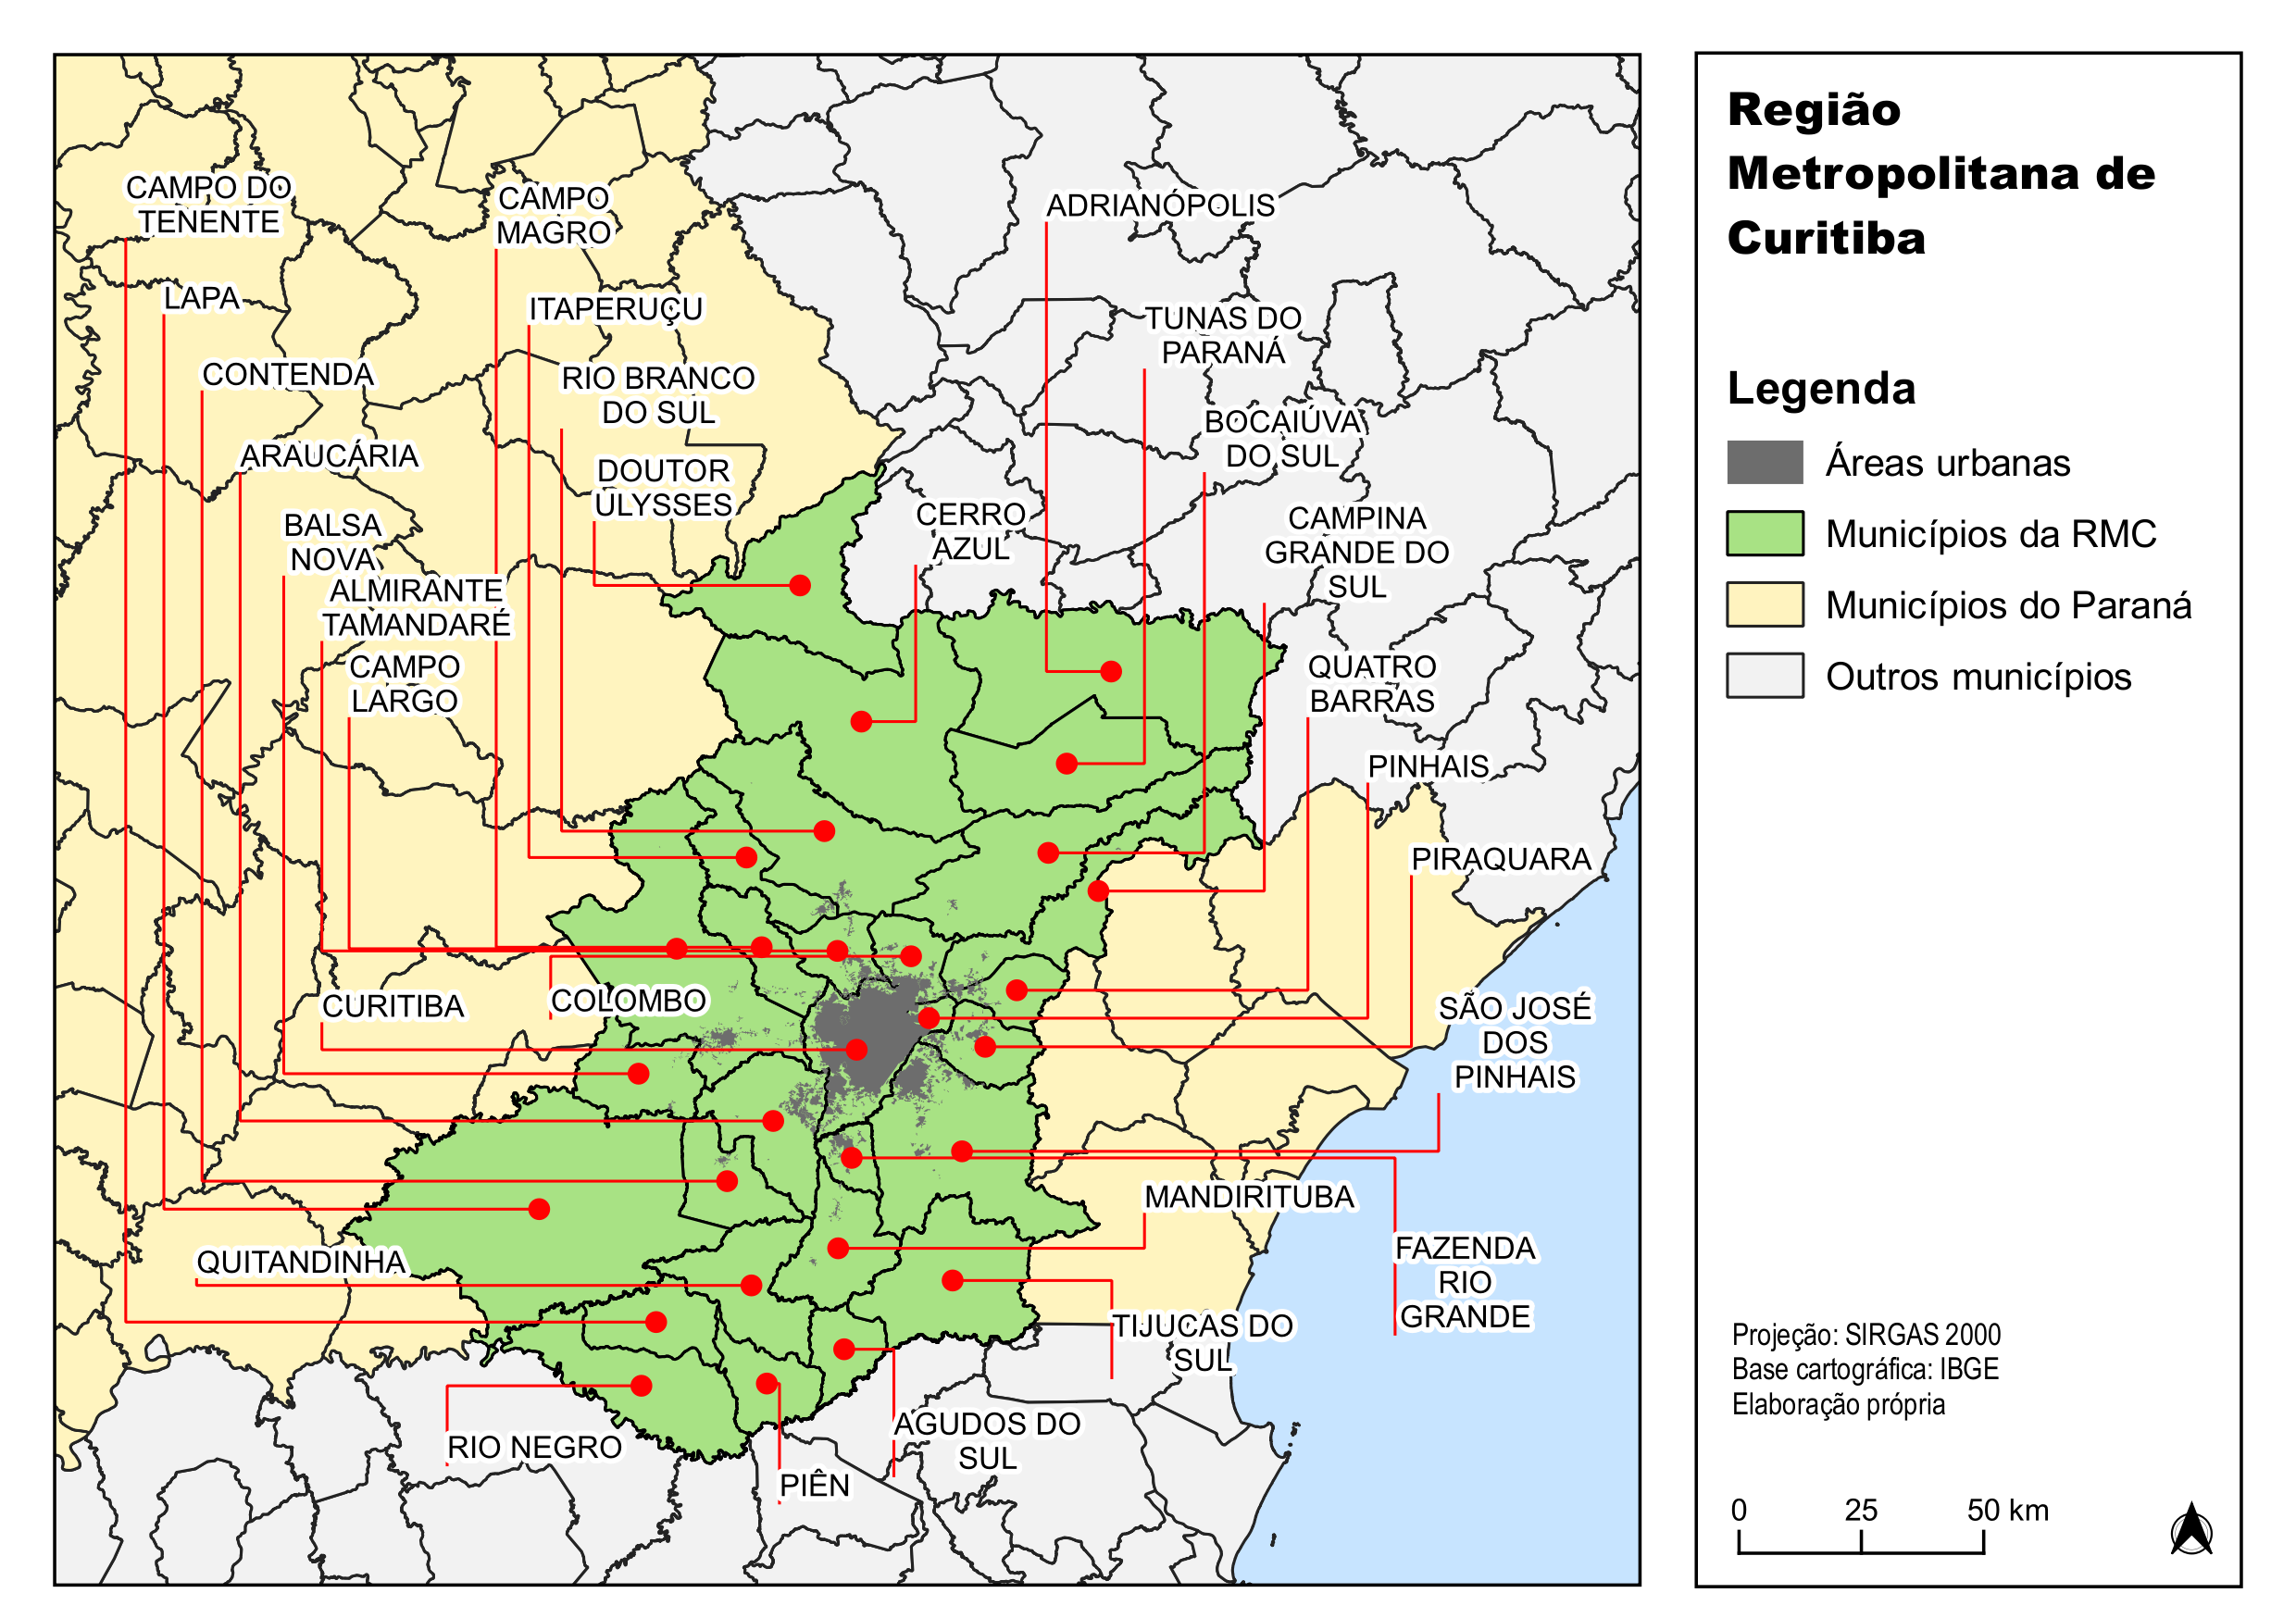
\includegraphics[width=0.85\linewidth]{../gis/produtos/RMC_config_atual}
			\legend{Elaboração própria}
		\end{figure}
	\end{landscape}

	\section{Dinâmica populacional}
	
	A RM de Curitiba reúne cerca de 27\% da população do Estado,  uma proporção menor que a média das regiões metropolitanas do país (38,61\%) (IBGE, 1991 e 1996), mas revela um  crescimento de 266,27\% em relação ao período inicial da aceleração do processo de urbanização regional, nos anos, (Lima, C., Mendonça, F., 2001, p., 140).
	
	Entre 1970 e 1980, o crescimento da RMC foi resultado de um movimento geral de metropolização do país e da elevada migração. Os censos mostram que a população da RM de Curitiba passou de 869.837 habitantes em 1970 (12,55\% da população do estado do Paraná) para 2.003.015 (23,7\%) em 1991.
	
	A partir da década de 1990, com o processo de construção de uma imagem da cidade por meio do marketing urbano, aliado a atração de investimentos, se deu o incremento populacional, alcançando ao ano 2000, 2.768.394 (28,95\% do estado) e 3.223.836 em 2010, ou 30,86\% do total estadual, dos quais 1.757.907 pertencem ao município-polo (16,78\% do total do estado) (IBGE, 2012a). Entre 2000 e 2010, o incremento populacional da região foi de 16,36\%, ou 453.364 pessoas a mais. Ao excluir Curitiba, as outras 28 cidades da RM apresentaram variação de 19,59\%, ou 288.305 novos habitantes.
	
	Segundo \citeonline[p. 64]{delgado2014a}, Curitiba é um exemplo nítido da organização social do trabalho e concentração do capital paranaenses, exacerbando um modelo de produção extremamente concentrador, sendo a configuração reforçada por políticas de desenvolvimento estaduais e também outras políticas de organização do espaço urbano, outrossim, para \citeonline[p. 4]{firkowski2002a} ``ao contrário do que se observa ao nível nacional com a desaceleração da concentração populacional nas regiões metropolitanas, no Paraná ocorre exatamente o oposto, ou seja, a exacerbação do movimento concentrador, principalmente na Região Metropolitana de Curitiba''.
	
	\begin{table}
		\centering
		\caption{Brasil, região Sul, Paraná, RM de Curitiba e municípios: estatísticas populacionais (2000-2010)}
		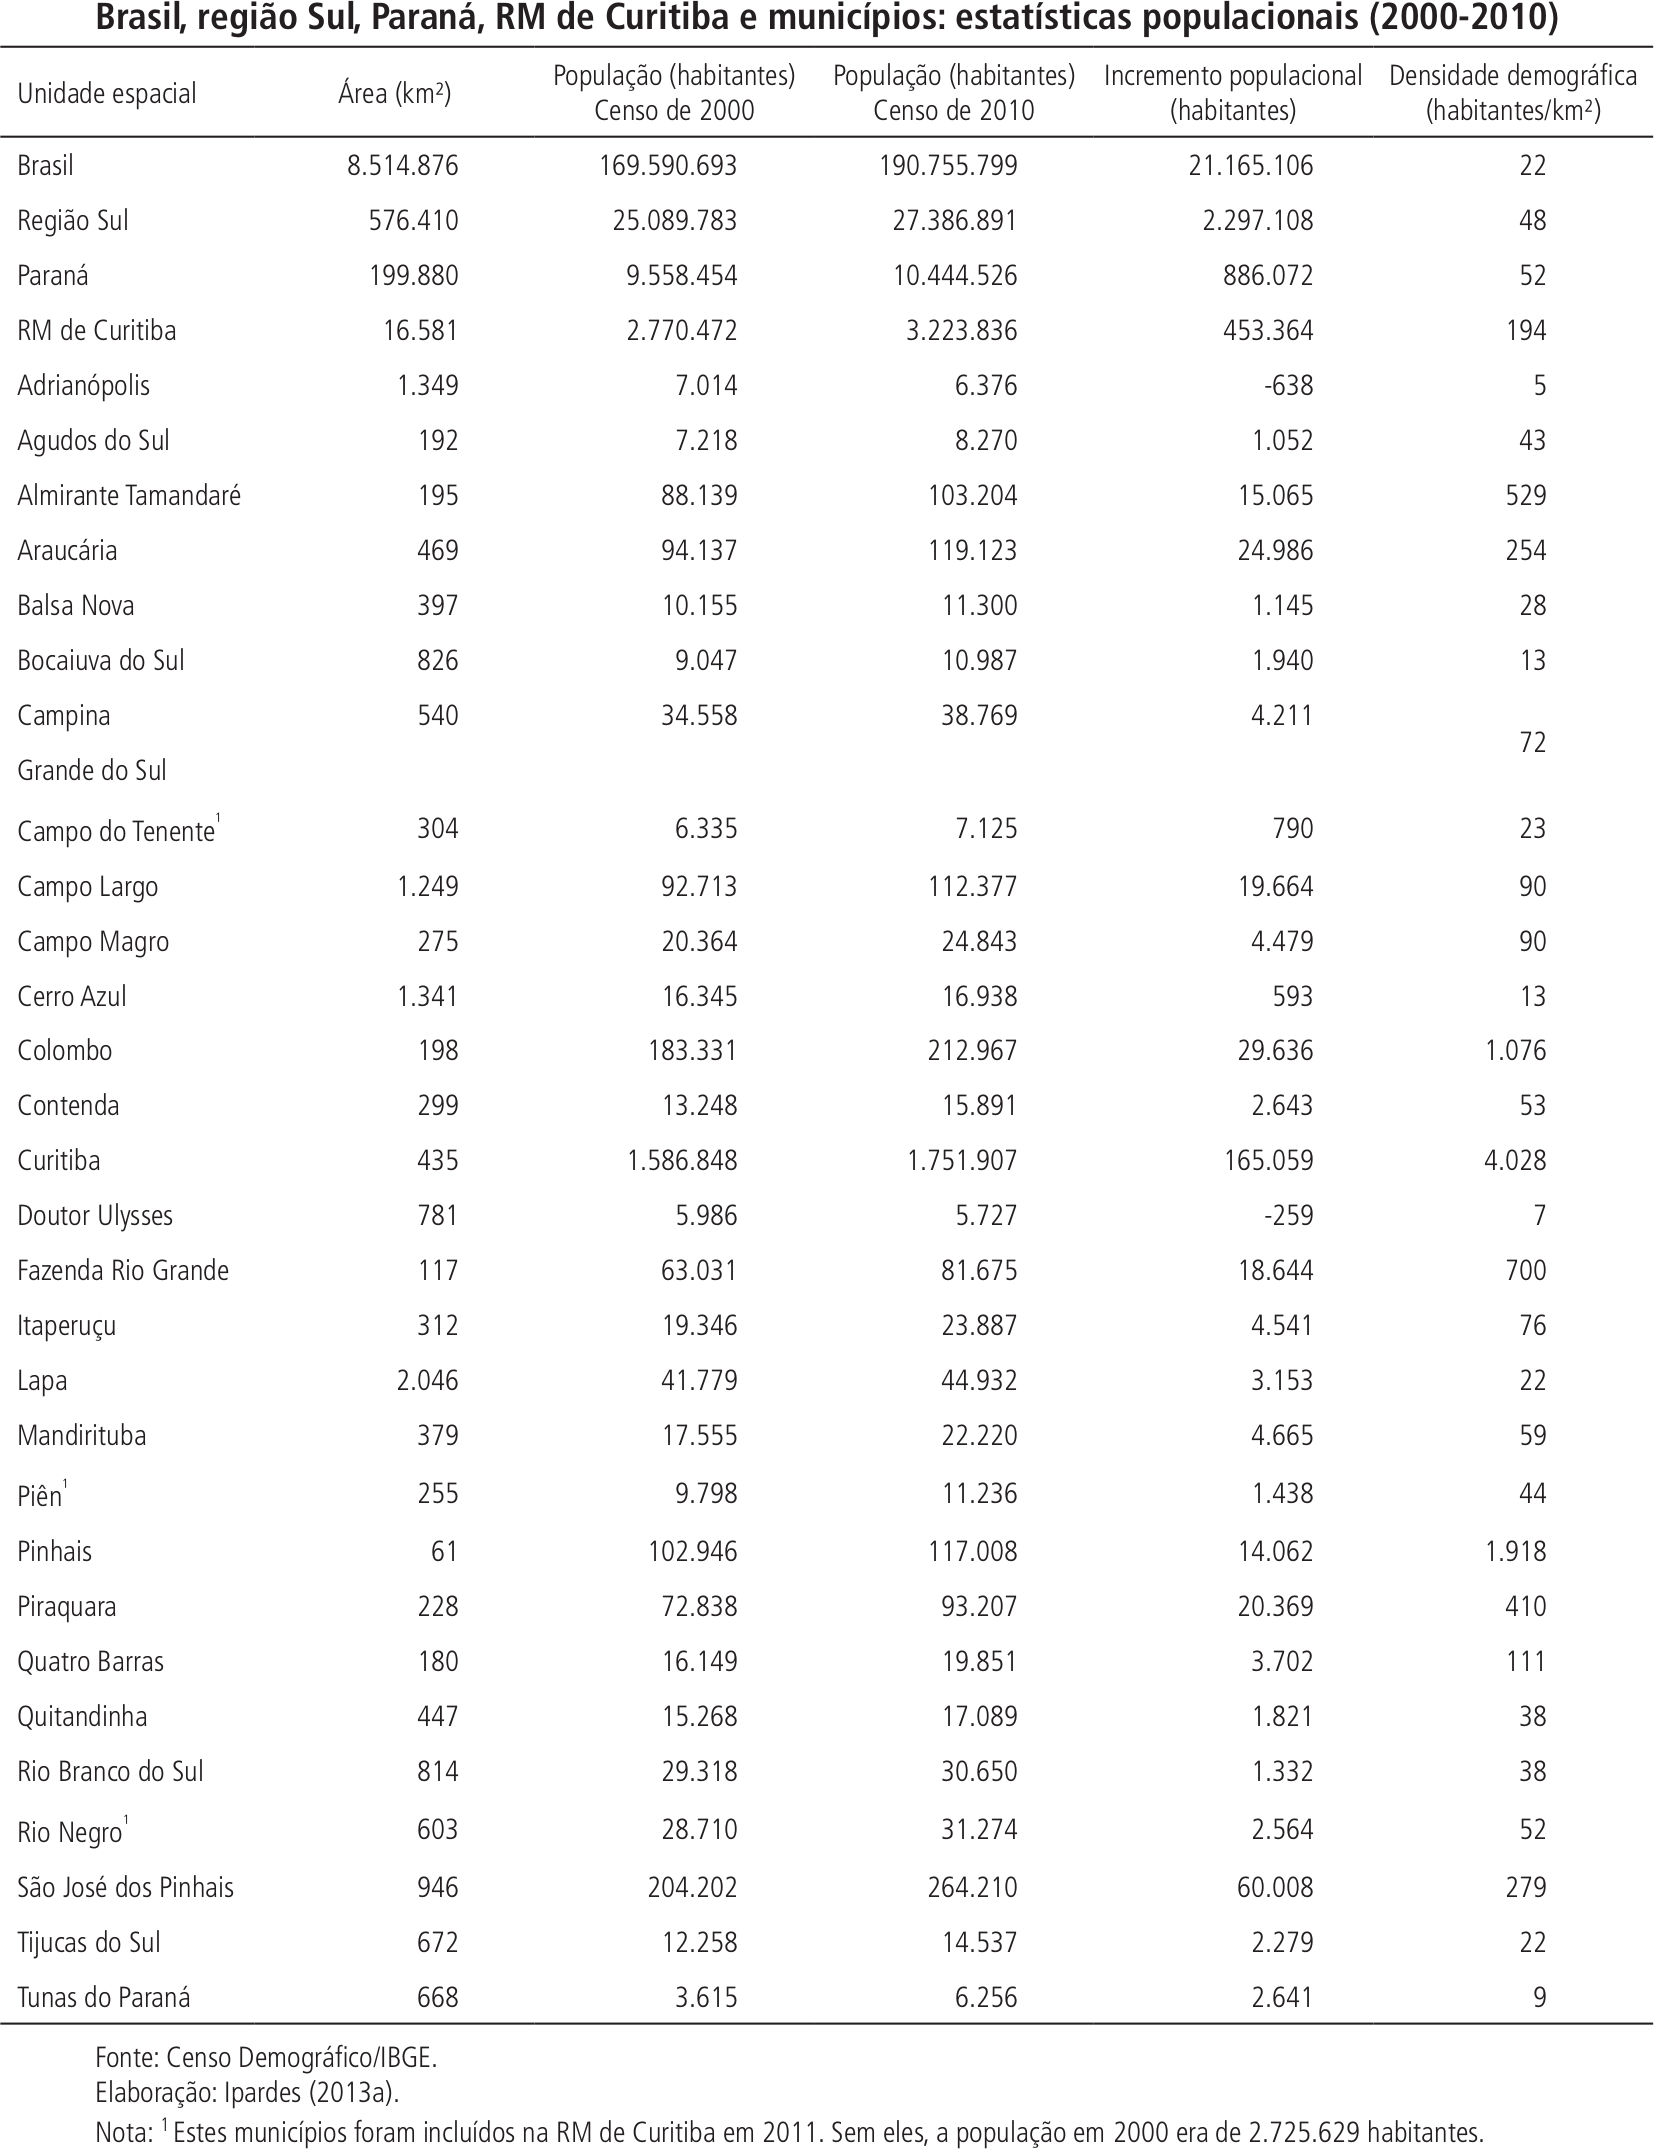
\includegraphics[width=1.0\linewidth]{img/costa2015a_01}
		\label{tab:costa2015a_01}
		\legend{Fonte: \citeonline[p. 9]{costa2015a}}
	\end{table}
	
	Mantidas as taxas atuais, as cidades da \gls{rmc} juntas tendem a se equiparar e/ou superar a  população de Curitiba antes da década de 2030. A \autoref{tab:costa2015a_01} apresenta as estatísticas populacionais para as décadas de 2000 e 2010, enquanto a \autoref{fig:costa2015a_02} apresenta um gráfico da dinâmica de crescimento populacional mencionada.
	
	\begin{figure}
		\centering
		\caption{RM de Curitiba e RM de Curitiba sem Curitiba: projeção populacional (1980-2023)}
		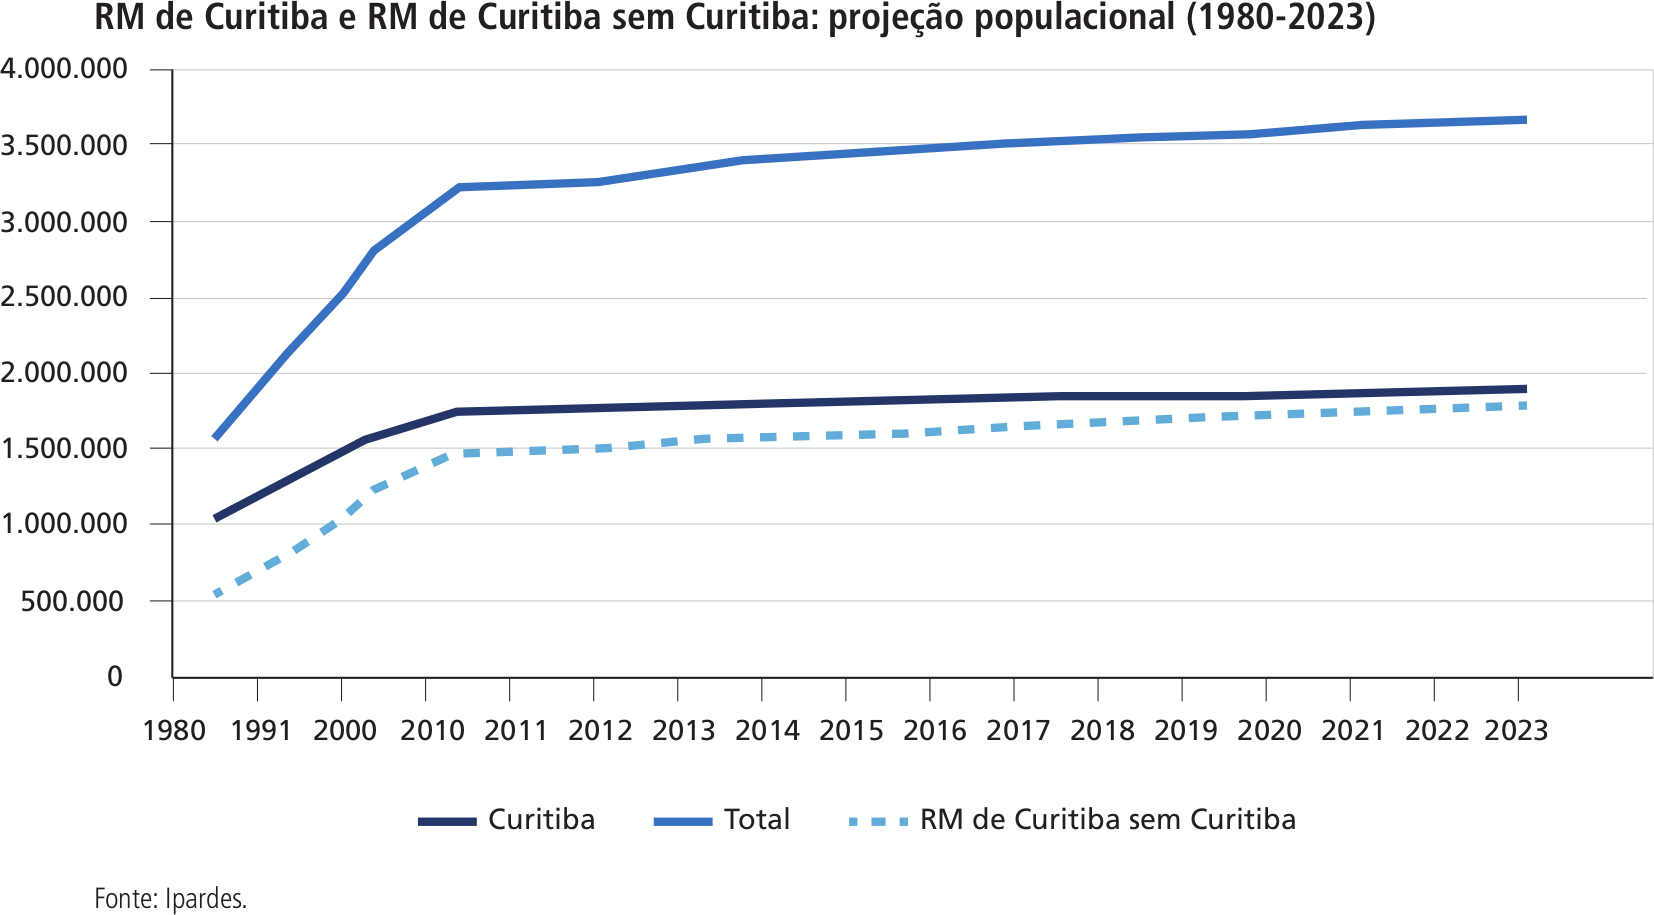
\includegraphics[width=1.0\linewidth]{img/costa2015a_02}
		\label{fig:costa2015a_02}
		\legend{Fonte: \citeonline[p. 10]{costa2015a}}
	\end{figure}
	
	% TODO precisa reescrever - é cópia do relatório - p. 9
	O conjunto de municípios se diferenciam entre si, em grau de integração ao fenômeno metropolitano, dividindo-se entre aqueles que de fato pertencem à aglomeração metropolitana (treze), que compõem o \glsdesc{nuc} (\gls{nuc}) (Comec, 2006; Ipardes, 2010), e aqueles formados pela maioria dos municípios, desmembrados ou inseridos na região por legislação estadual.
	
	% TODO precisa reescrever - é cópia do relatório - p. 10
    De acordo com dados do Ipardes (2005), o extravasamento da população sobre os municípios do NUC foi iniciado na década de 1970, abrangendo inicialmente as áreas ao norte do município e as áreas contínuas ao polo, originando vazios entre estas áreas e as sedes municipais. As extensões limítrofes conurbadas de Almirante Tamandaré, Araucária, Campo Largo e Colombo, e a distância que possuem de suas sedes municipais, exemplificam este fato.
	
	\begin{figure}
		\centering
		\caption{Mapa do NUC (2012)}
		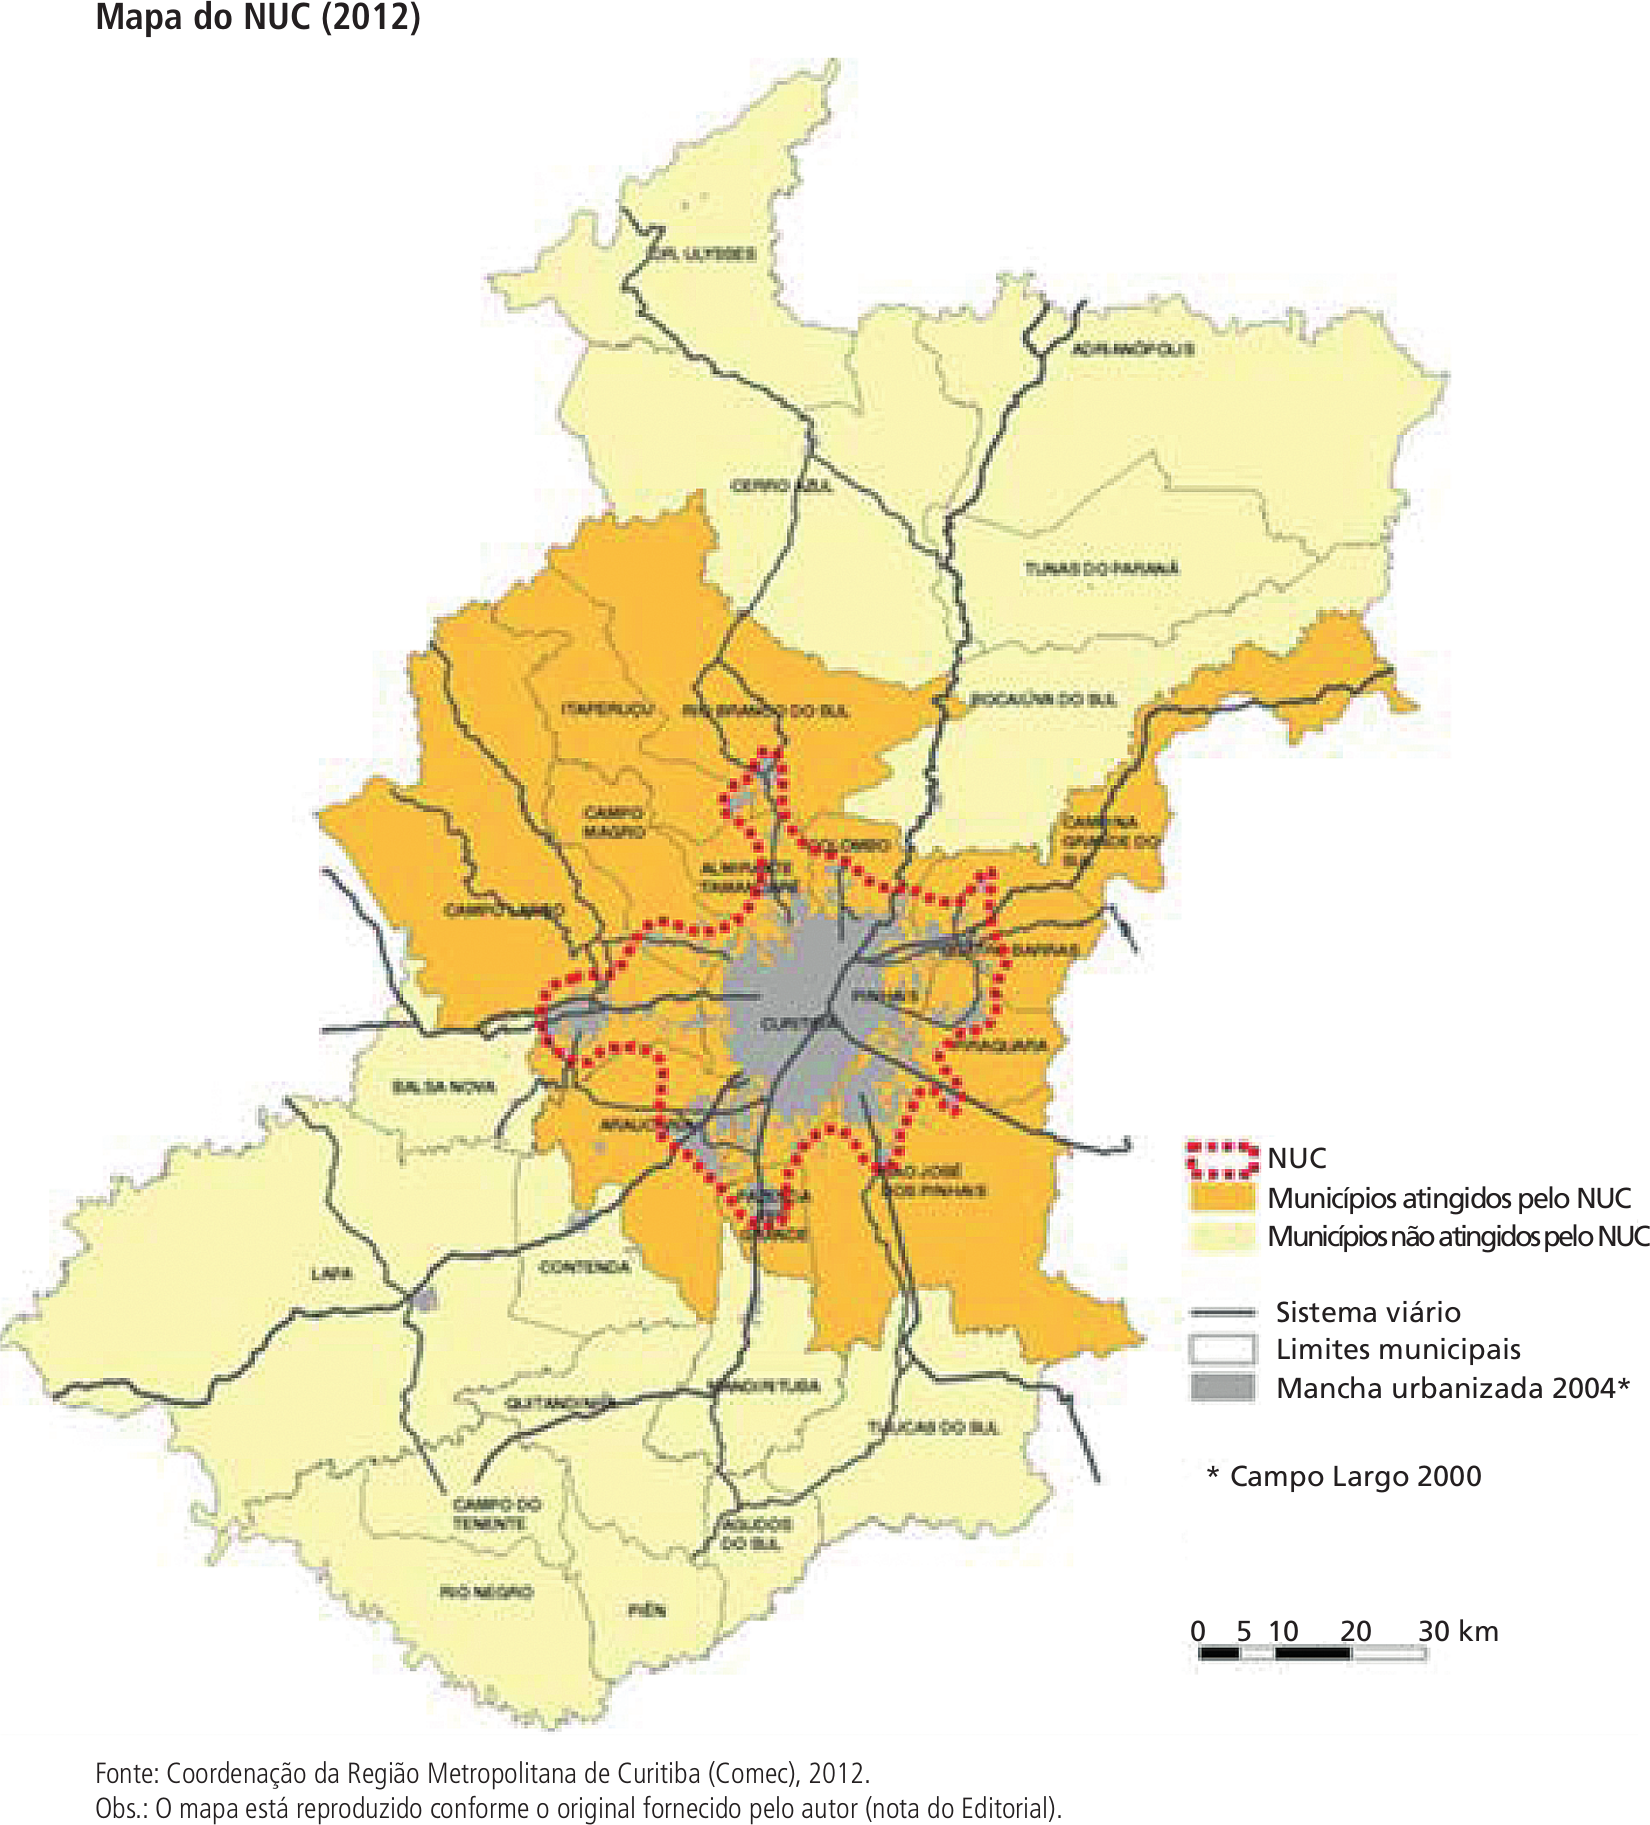
\includegraphics[width=1.0\linewidth]{img/costa2015a_03}
		\label{fig:costa2015a_03}
		\legend{Fonte: \citeonline[p. 11]{costa2015a}}
	\end{figure}
    
    % TODO precisa reescrever - é cópia do relatório - p. 11
    A expansão do crescimento curitibano tem sido direcionada para a porção sul e para as áreas de divisa da cidade. Esta afirmação é confirmada pelos dados do Censo de 2010, que apresentam os dez bairros de Curitiba com maior incremento populacional no período 2000-2010.
    
	\begin{figure}
		\centering
		\caption{Bairros com maior incremento absoluto populacional (2000-2010)}
		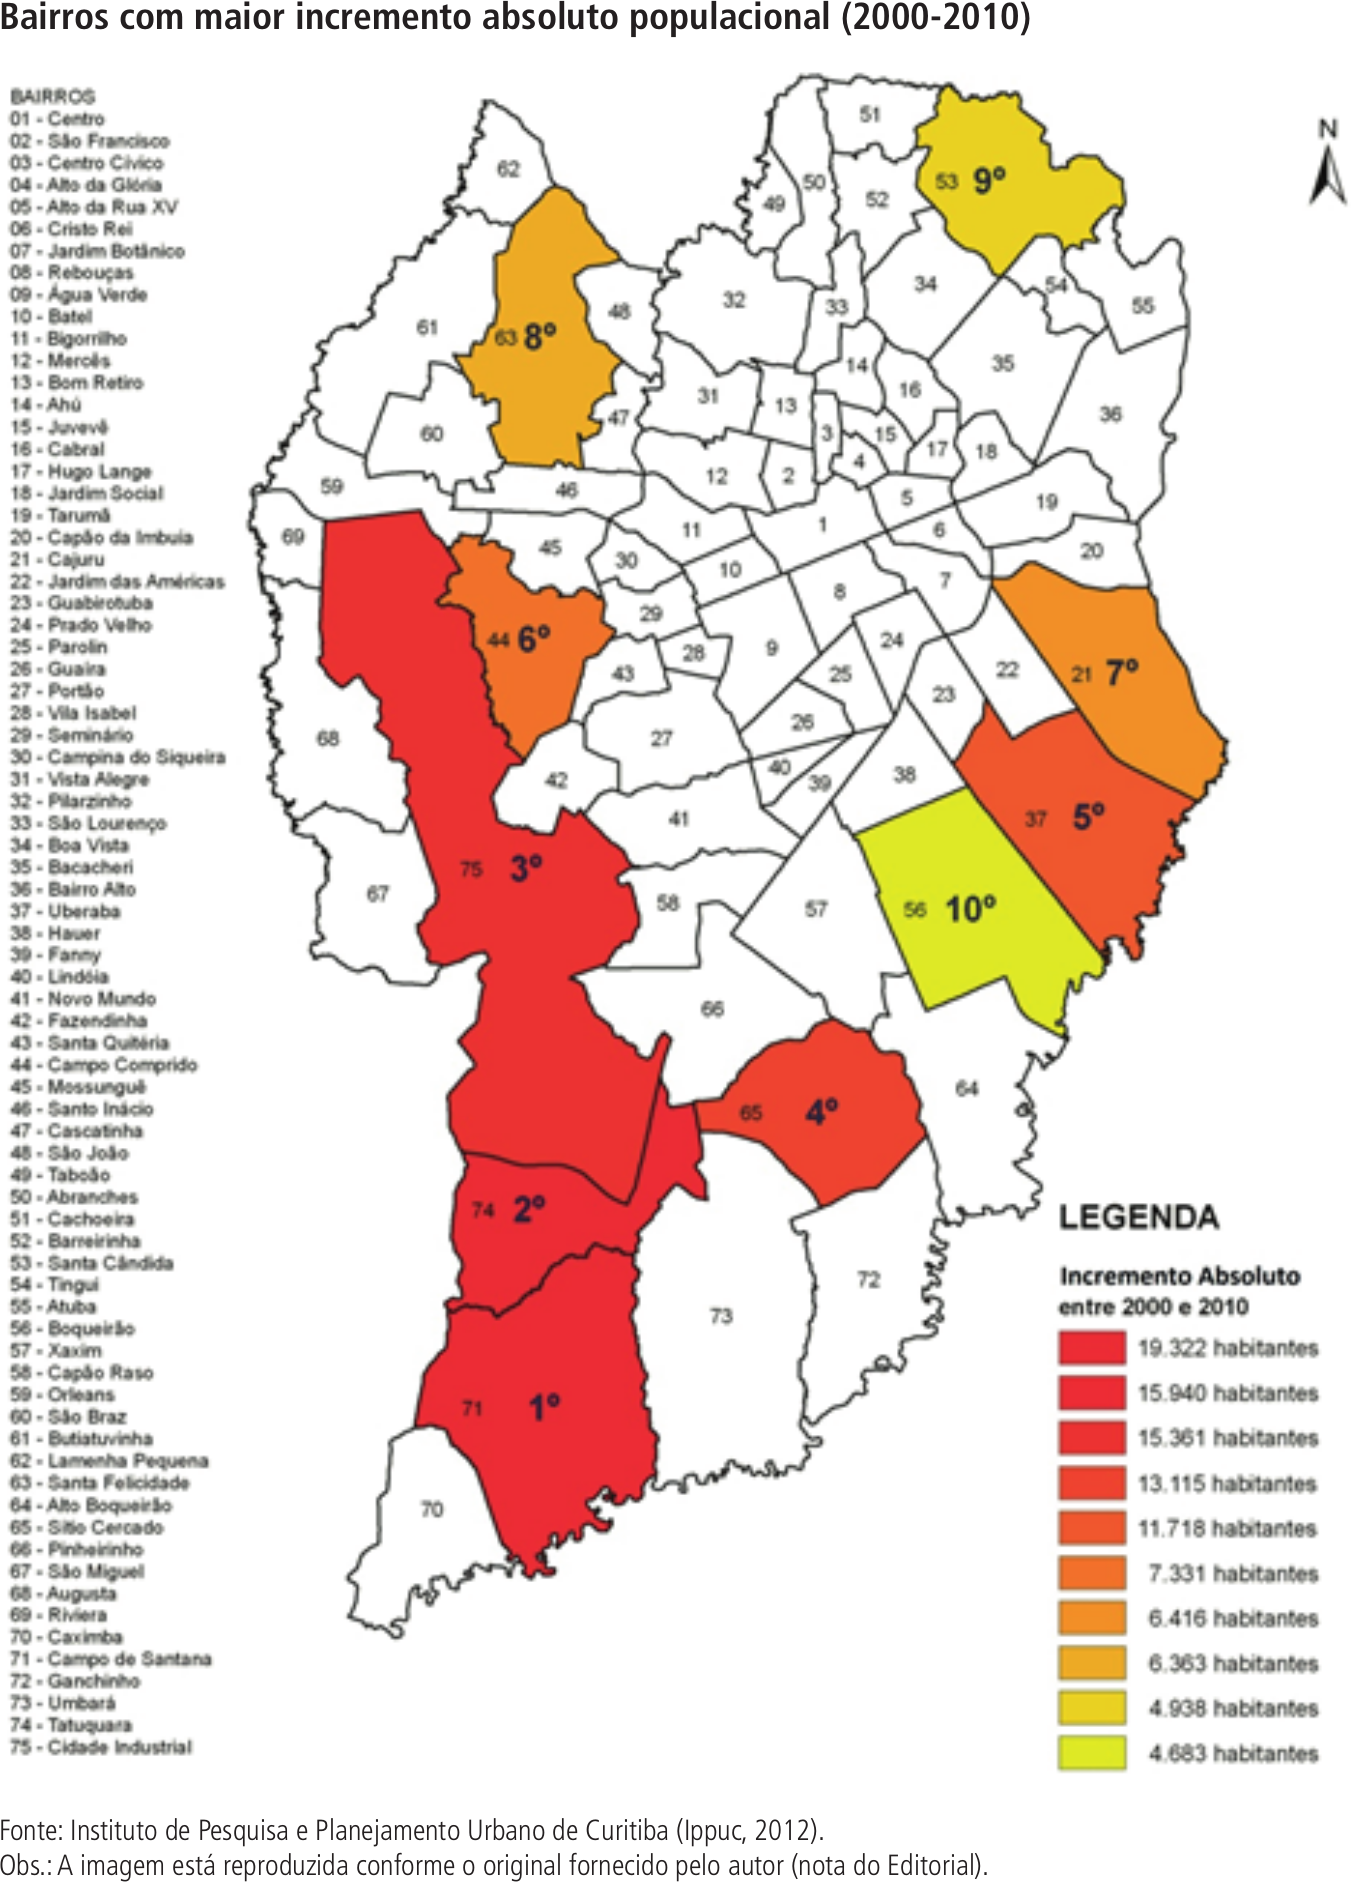
\includegraphics[width=1.0\linewidth]{img/costa2015a_04}
		\label{fig:costa2015a_04}
		\legend{Fonte: \citeonline[p. 12]{costa2015a}}
	\end{figure}
    
	\section{Meio físico}
	
	% TODO - mais copia e cola: p. 30 do relatório do IPEA	
	Segundo consta em estudos do IPEA, a legislação que versa sobre os recursos hídricos e proteção ambiental tem largo alcance na gestão da RM de Curitiba. Além da legislação federal, a legislação estadual possui uma série de documentos que fazem referência a esta função, como o Decreto Estadual no 6.194/2012 que declara as áreas de interesse de mananciais de abastecimento público. Contudo, a principal lei ligada aos recursos hídricos e proteção ambiental é a Lei Estadual no 12.248/1998. A Lei número 12.248/1998, conhecida como ``Lei dos Mananciais'', adota novos conceitos de gestão do uso e ocupação do solo dos mananciais da RM de Curitiba e concebe, a partir de necessidades identificadas, o ``tratamento diferenciado de áreas de manancial sob pressão por ocupação, compartilhamento do processo de decisão, entre estado e municípios, e a necessidade de um efetivo monitoramento e fiscalização do uso e ocupação do solo'' (Comec, 2013a). Entre outras inovações, esta Lei levou à criação do Sigprom, focado em variáveis de uso e ocupação do solo, buscando garantir, recuperar e preservar as características e condições necessárias para a manutenção dos mananciais para abastecimento. Os mecanismos de ação do Sigprom na gestão do uso e ocupação são, entre outros, as UTPs e APAs (que aglutinam áreas de diferentes municípios que devem ser trabalhadas em conjunto), o CGM (seu órgão máximo), que serão detalhados a seguir, além do Plano de Proteção Ambiental e Reordenamento Territorial (Ppart) em Áreas de Proteção aos Mananciais e do FPA, detalhado na seção 5. Entre os principais instrumentos de gestão, as UTPs são áreas de uso restritivo, ambientalmente frágeis, especialmente as do leste metropolitano, onde estão os mananciais e que estavam sendo sistematicamente ocupadas irregularmente há quase uma década. Os recortes territoriais das UTPs recebem zoneamento especial, de forma a reordenar o uso e ocupação do solo. Foram implantadas cinco UTPs na região.
	
	\begin{landscape}
		\begin{figure}
			\centering
			\caption{Unidades de conservação e hidrografia da \glsdesc{rmc}}
			\label{fig:rmcconservacao}
			\includegraphics[width=0.85\linewidth]{../gis/produtos/RMC_unid_conservacao}
			\legend{Elaboração própria}
		\end{figure}
	\end{landscape}
	
	\section{Mobilidade pendular}
	
	% TODO - mais cópia do relatório a ser reescrita - p. 12
	Quanto à capacidade de movimentação no espaço metropolitano, a mobilidade auferida pelo Censo de 2010 mostra que na RM de Curitiba, 384.754 pessoas (16,1\%) deslocavam-se do município de residência para estudar e/ou trabalhar em outro município, entre as 2,4 milhões de pessoas que estudavam e/ou trabalhavam. O principal motivo, segundo o Instituto Brasileiro de Geografia e Estatística (IBGE), era o trabalho. Dos 1.657.198 trabalhadores residentes na RM de Curitiba, 318.298 exerciam sua atividade em município diferente do de residência, o que corresponde a 19,2\%; para os moradores de Curitiba, o percentual de deslocamentos para outros municípios é de 6,3\% (Cintra, Delgado e Moura, 2012). Esta dinâmica se mostra acentuada entre os municípios integrantes do NUC, ainda que novos municípios tenham se integrado de forma incipiente à complexidade deste, conforme a figura abaixo.
	
	\begin{figure}
		\centering
		\caption{RM de Curitiba: fluxo de entrada para trabalho (2010)}
		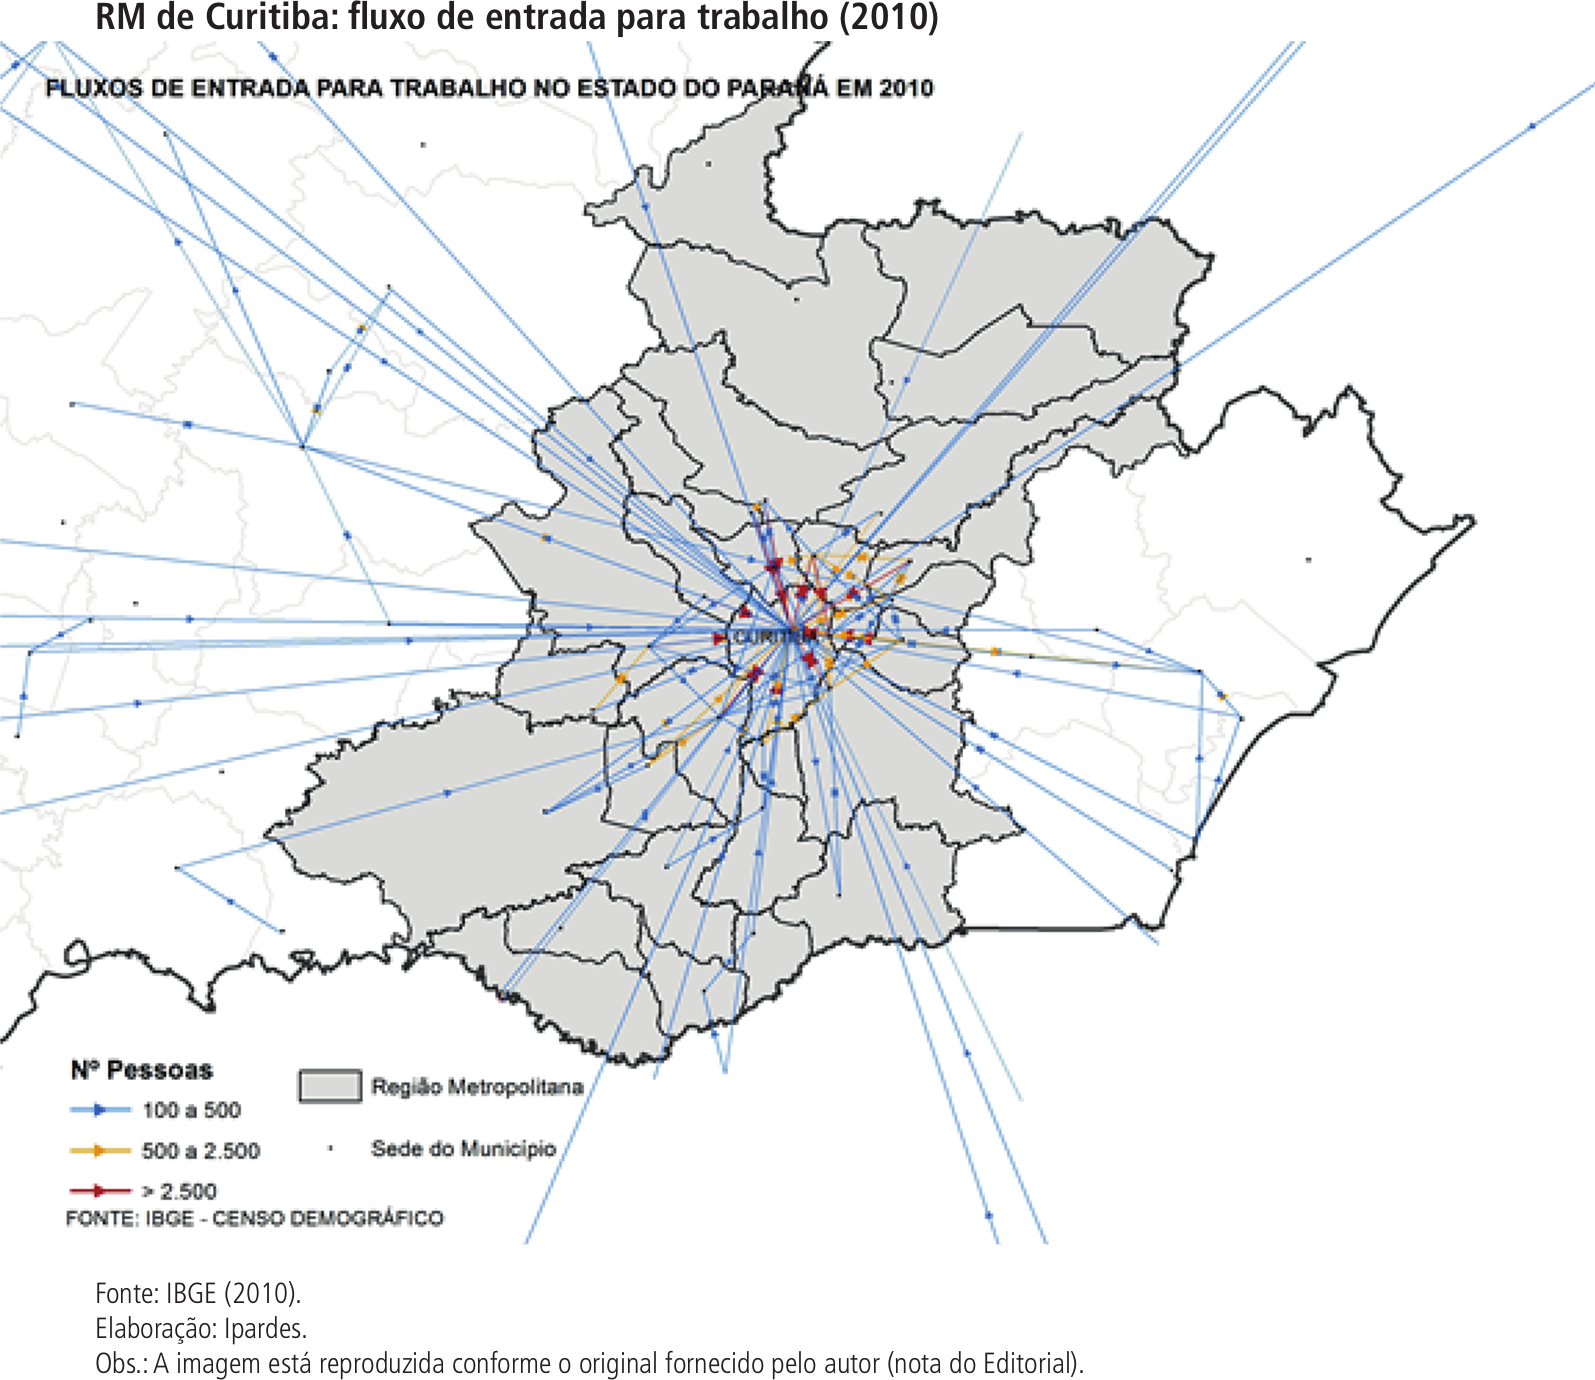
\includegraphics[width=1.0\linewidth]{img/costa2015a_05}
		\label{fig:costa2015a_05}
		\legend{Fonte: \citeonline[p. 14]{costa2015a}}
	\end{figure}

	\begin{figure}
		\centering
		\caption{RM de Curitiba: fluxo de saída para trabalho (2010)}
		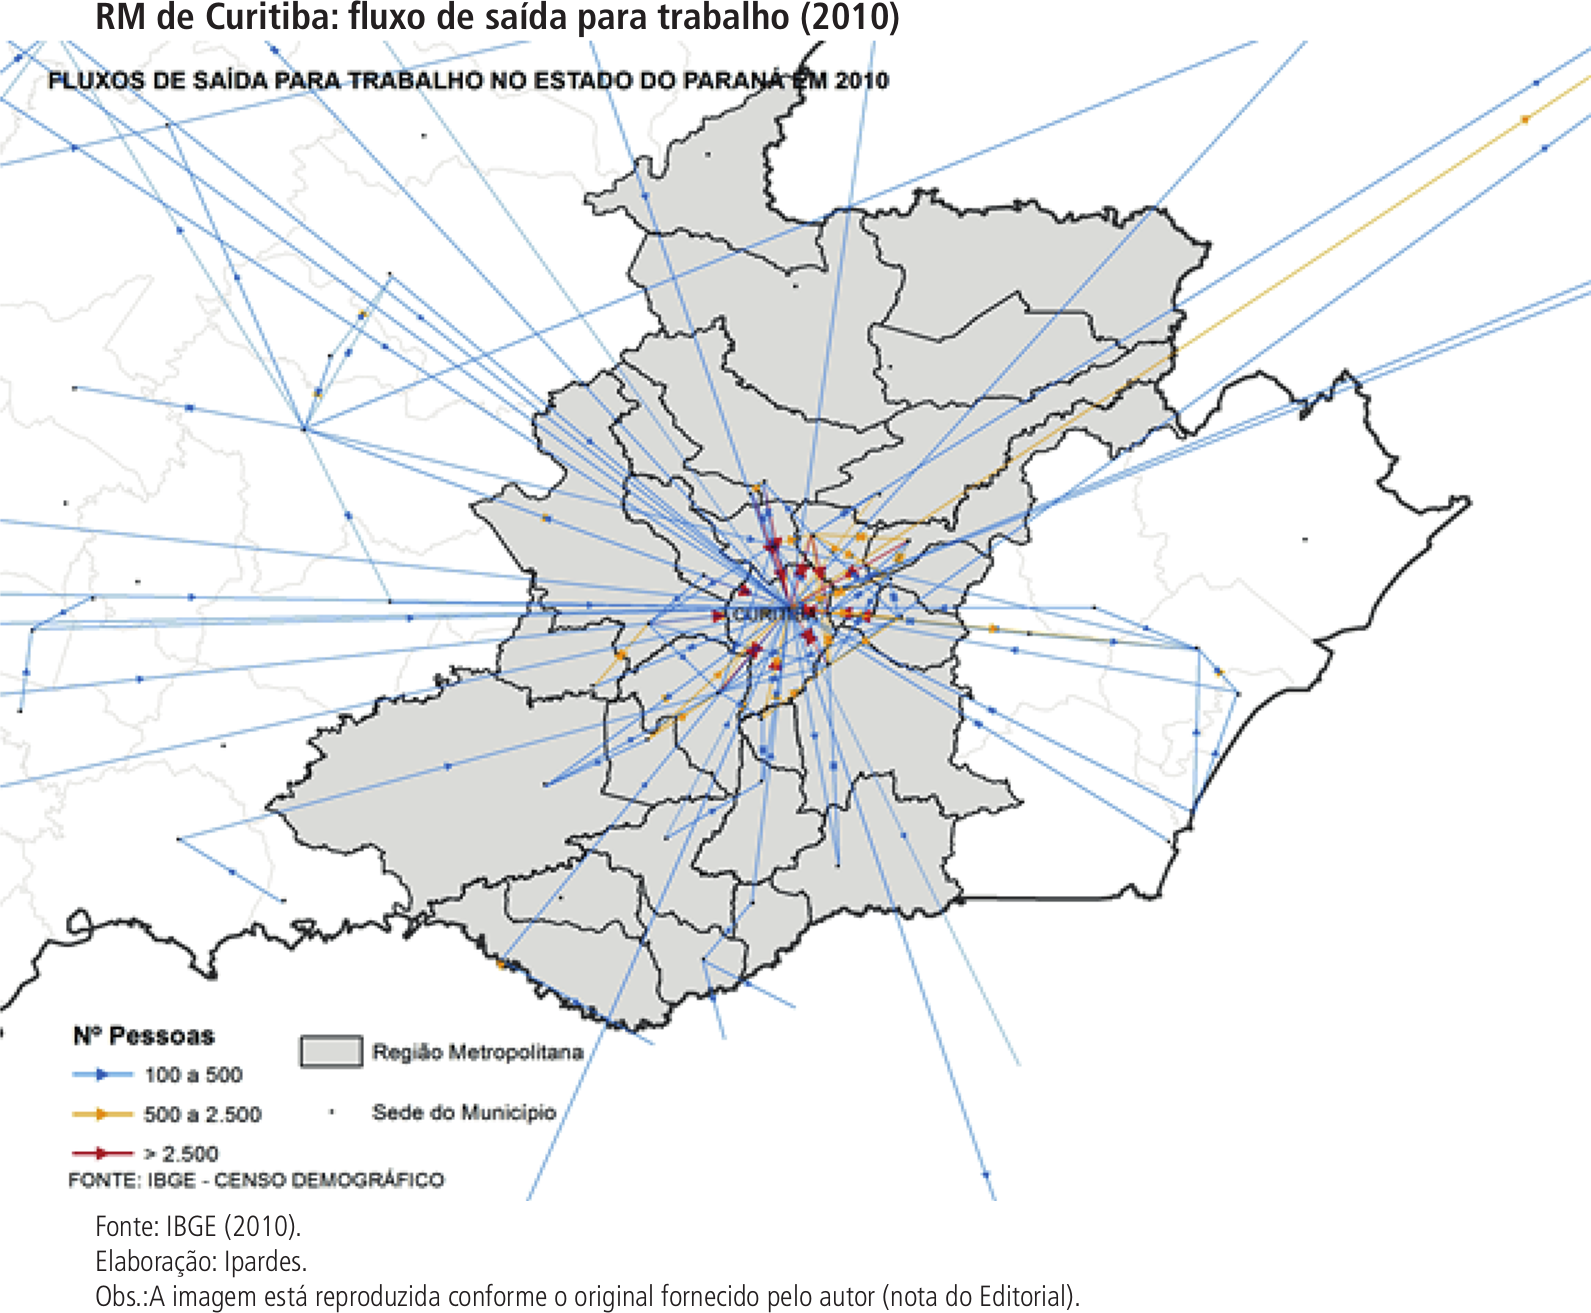
\includegraphics[width=1.0\linewidth]{img/costa2015a_06}
		\label{fig:costa2015a_06}
		\legend{Fonte: \citeonline[p. 14]{costa2015a}}
	\end{figure}
	
	\begin{figure}
		\centering
		\caption{RM de Curitiba: fluxo de entrada para estudo (2010)}
		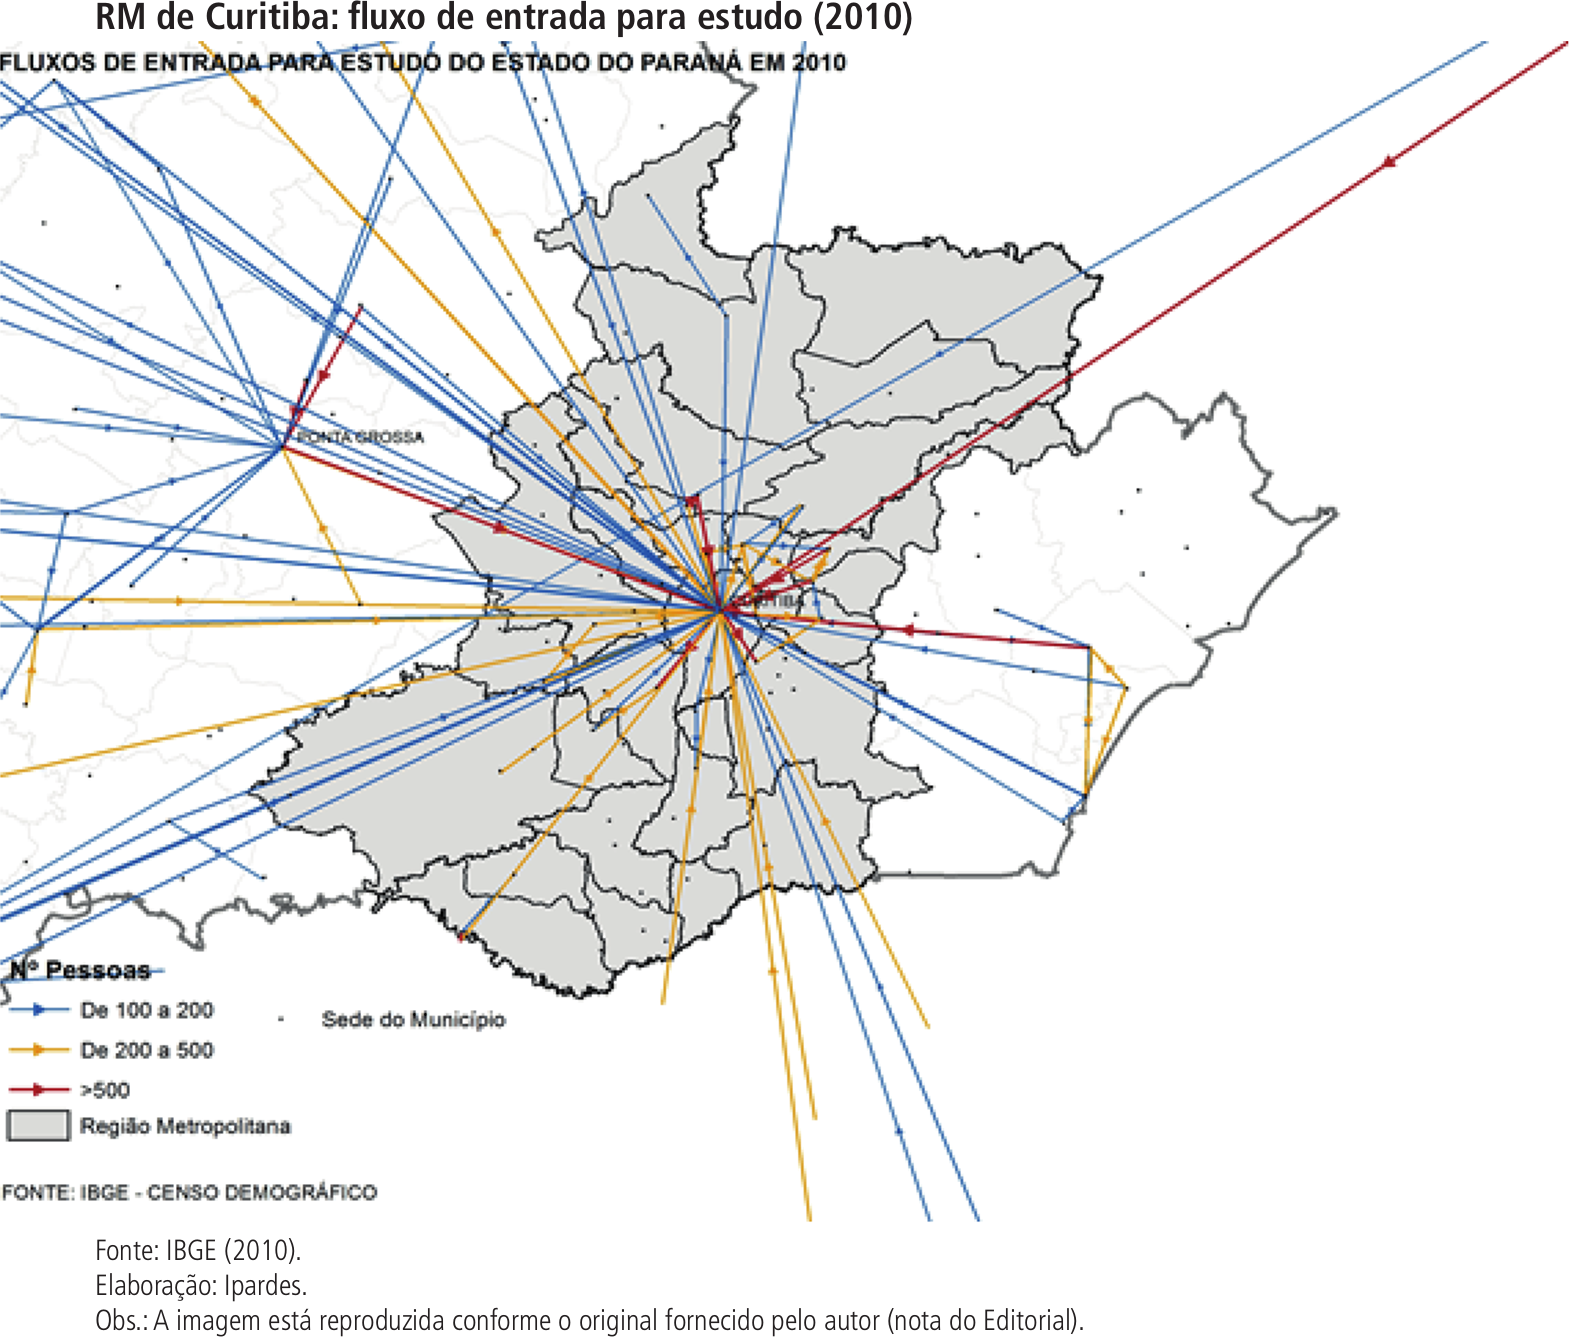
\includegraphics[width=1.0\linewidth]{img/costa2015a_07}
		\label{fig:costa2015a_07}
		\legend{Fonte: \citeonline[p. 15]{costa2015a}}
	\end{figure}

	\begin{figure}
		\centering
		\caption{RM de Curitiba: fluxo de saída para estudo (2010)}
		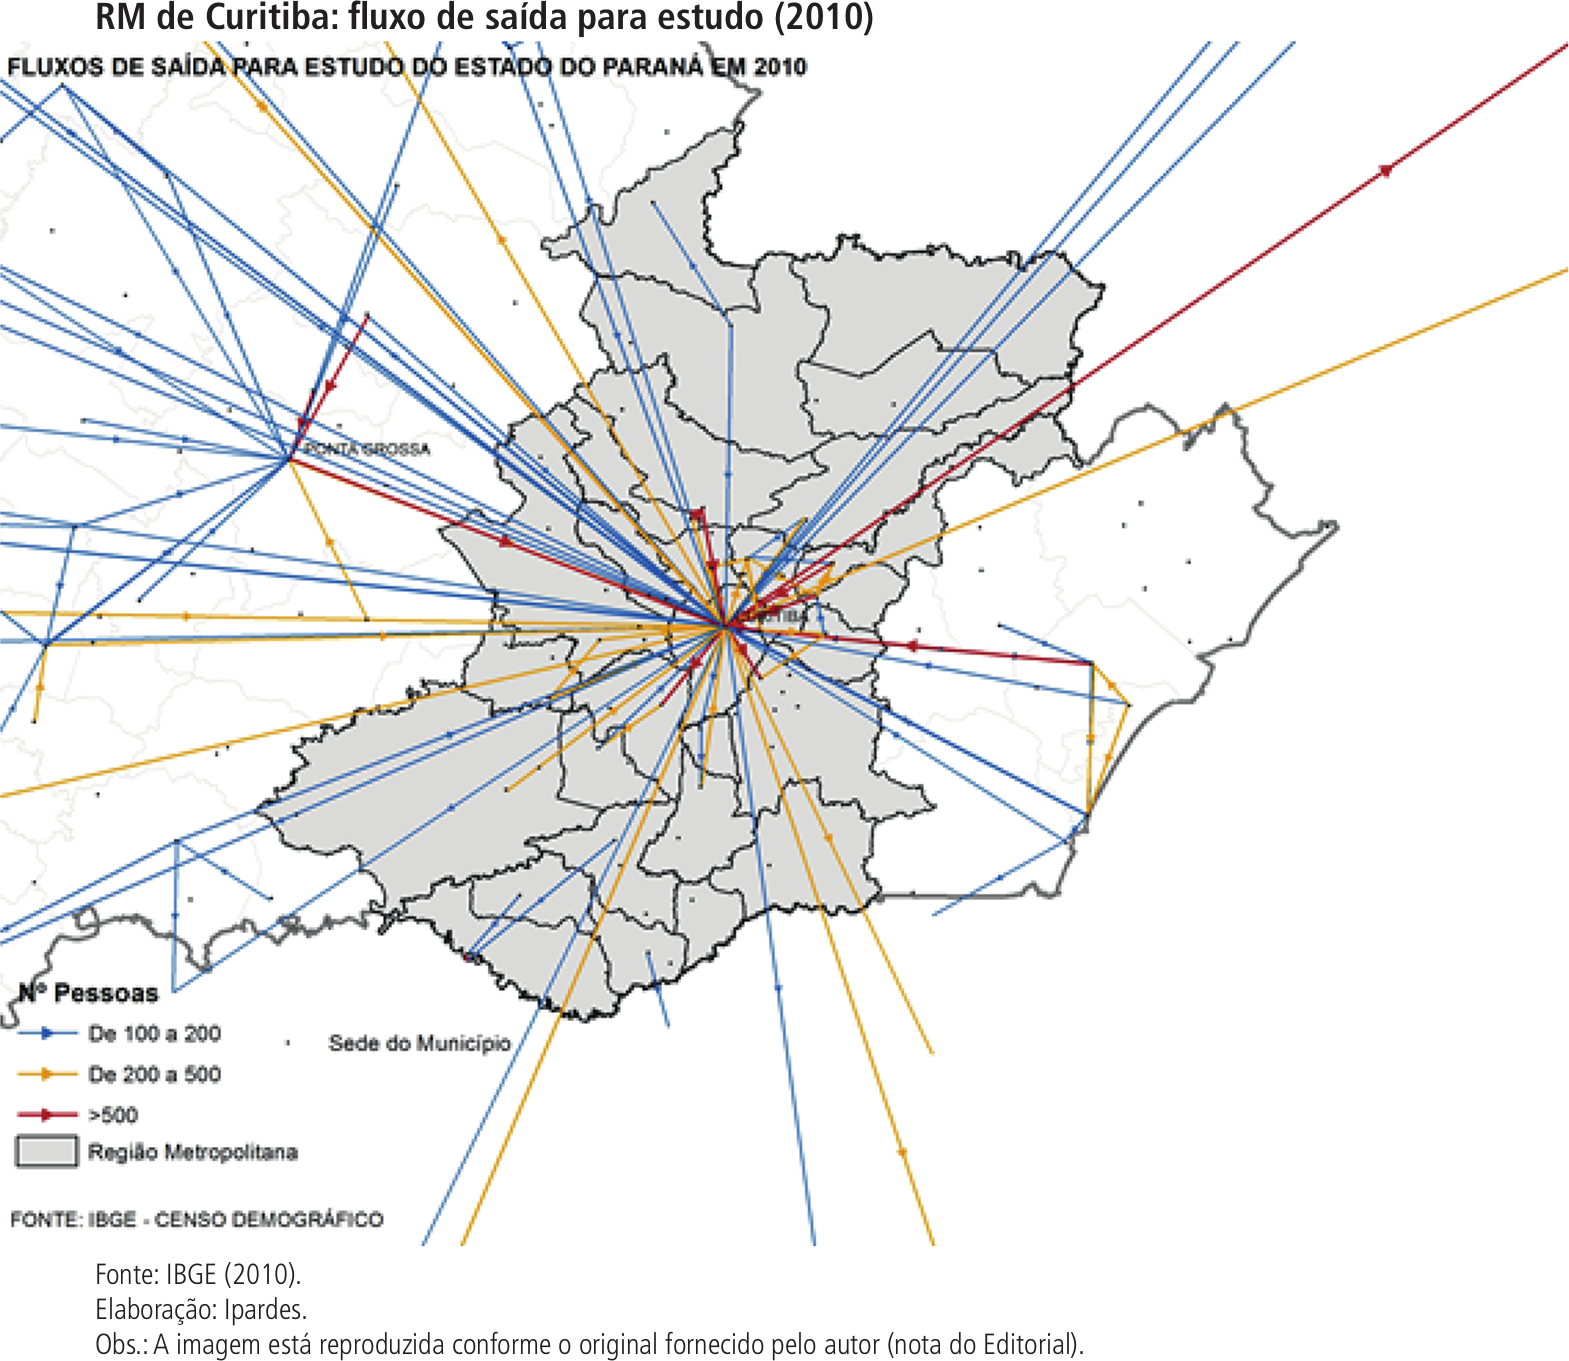
\includegraphics[width=1.0\linewidth]{img/costa2015a_08}
		\label{fig:costa2015a_08}
		\legend{Fonte: \citeonline[p. 15]{costa2015a}}
	\end{figure}
	
	% TODO - mais cópia - p. 15
	Os maiores fluxos de deslocamentos pendulares se dão entre as principais centralidades da rede urbana, e, ainda que multidirecional, a RM de Curitiba é o espaço no estado do Paraná onde as relações entre municípios possuem maior abrangência e intensidade.
	
	\section{Aspectos Econômicos}
	
	As décadas de 70 e 80 foram marcadas por uma concentração industrial no município de Curitiba (\glsdesc{cic} - \gls{cic}), e uma área adjacente que atingia o município de Araucária, em seu centro industrial (\gls{ciar}). No entanto, seu padrão se dava de forma dispersa no interior de ambos. Já na década de 90, a indústria se mostra desconcentrada no espaço urbano ampliado e mais concentrada no interior de alguns distritos. Apesar do processo de desconcentração, iniciado nos anos 70, a \gls{rmc} segue sendo o destino das principais capitais industriais, como também das pessoas. 
	
	São José dos Pinhais é apontado (Firkowski, 2002) como um indicador importante de mudanças na localização das indústrias, uma vez que apresenta uma inversão no padrão, pois o vetor de expansão fomentado sempre foi localizado à oeste, e São José dos Pinhais se encontra em direção contrária, a Leste. E é nessa região que predomina a concentração das indústrias, revelando conflitos importantes em relação ao uso do solo e questão ambiental, além de se especializarem de modo seletivo na \gls{rmc}, devendo ser ressaltado aqui a importância de se distinguir os limites da Região Metropolitana institucionalizados (26 municípios) e do aglomerado metropolitano (12 municípios). 
	
	Trata-se aqui de indústrias referentes a um mesmo processo produtivo, em que muitas são fornecedoras das indústrias automobilísticas, cuja ocupação não está na mesma planta, porém estão em suas proximidades. Este tipo de indústria produz um território específico, os distritos industriais, que são bem diferentes da formação do passado, baseado, sobretudo, no modelo de acumulação flexível. A localização de uma grande empresa não se faz independente e sozinha, como podia ocorrer no passado. A Volvo, quando se instalou em Curitiba no final da década de 70, não desencadeou a vinda de outras empresas no ritmo e velocidade com que isso ocorre na atualidade. Da mesma forma, sua localização se deu no interior de uma grande área industrial – um distrito industrial sob a ótica do uso do solo urbano, uma área reservada para uso industrial –, onde seus vizinhos não eram necessariamente do mesmo setor de atividade e tampouco complementares à sua produção.
	
	Atualmente, a inserção da indústria automobilística forma um tipo de distrito industrial ``fechado'', isto é, um complexo de produção flexível, cuja estratégia de localização é definida pela montadora e acompanhada pelos fornecedores. Ao serem observados os locais escolhidos pelos complexos de produção da indústria automobilística, veremos que estes se localizam preferencialmente onde as marcas de um forte passado industrial são praticamente inexistentes, e onde os novos métodos flexíveis de produção e organização da empresa não encontram barreiras físicas, sociais ou trabalhistas. Os novos locais escolhidos como o caso de Curitiba, são marcados como o novo, o que está por ser construído e não predeterminado por enclaves ou resistências. Além disso, somam-se a isso outros fatores, como o meio inovador, tecnologias, infra-estrutura específica como a rede de fibra óptica, diversidade de sinergias possíveis, parcerias, concentrações imateriais, dentre outros) e atores, tendo em vista que a escolha de uma localização não se dá unicamente pela supremacia das considerações técnicas e econômicas, mas também pelas oportunidades. 
	
	Essa estrutura de produção flexível carrega significativos entraves socioespaciais, sendo os ambientais os mais relevantes, dado o fundamento da escolha de localização pelos grandes grupos econômicos e a subordinação dos governos locais e estaduais em atender prontamente às demandas impostas, com receio de deixar escapar o capital para outras áreas.
	
	\begin{citacao}
		(...) em todos os níveis da questão ambiental existem interesses conflitantes e, portanto, custos a serem alocados a determinados setores ou determinadas sociedades”, e quando o que está em jogo é a localização de grandes empresas, tais custos tendem a ser socializados pela população da área receptora desses capitais, mesmo que, num primeiro momento, ela não se dê conta de quão alto eles serão no futuro. (Martine, 1993, p. 38, citado por Firkowski, 2002) 
	\end{citacao}

	\chapter{Funções públicas de interesse comum}
	
	\section{Recursos hídricos e proteção ambiental}
	
	\section{Saneamento básico}
	
	\section{Transportes e sistema viário}
	
	A luz do que introduz \citeonline[p. 375]{paese2014a}, o planejamento urbano da capital é especialmente marcante devido à década de 1970 e a implantação de um sistema de transporte coletivo sobre pneus baseados em linhas expressas de ônibus, que atualmente operam com veículos biarticulados em vias segregadas. A inserção das vias segregadas se dá a partir de uma lógica de eixos trinários radiais (centro-bairro/bairro-centro), que contribuíram para estruturar o adensamento construtivo e a verticalização:
	
	\begin{citacao}
		O planejamento urbano de Curitiba, implantado a partir da década de 1970, possui o sistema de transporte como um de seus pilares. Os eixos trinários, compostos por duas vias rápidas de ligação centro--bairro e bairro-centro, contendo ao centro uma canaleta exclusiva para o ônibus expresso (atualmente transformado em biarticulado), foram os grandes estruturadores da expansão urbana, em razão do que tais eixos foram também definidos como locais preferenciais de verticalização e de expansão linear do centro, induzindo o uso, na parte inferior dos edifícios residenciais, de atividades de comércio e serviços.
	\end{citacao}

	No âmbito de uma discussão de caráter metropolitano, \citeonline[p. 376]{paese2014a} tratam com a naturalidade à incorporação dos municípios do entorno ao sistema de transporte, cujos eixos originalmente foram concebidos restritos aos limites da capital. A incorporação dá origem à \glsdesc{rit} (\gls{rit}):
	
	\begin{citacao}
		As linhas que constituem a RIT são as que podem estabelecer integração físico-tarifária em terminais ou estações com o Sistema de Transporte de Curitiba. É caracterizada por apresentar uma hierarquia de tipos de linhas de ônibus, podendo estar vinculadas a um terminal ou não. As linhas vinculadas a terminais de transporte ou estações--tubos estabelecem uma integração físico-tarifária na qual o passageiro, pagando apenas uma tarifa, pode descer de um ônibus e ingressar em outro que também esteja vinculado ao terminal ou estação-tubo. Os terminais e estações-tubo estão localizados nos municípios integrados, nas vias expressas do sistema de Bus Rapid Transit (BRT) e em outras importantes vias de Curitiba e municípios mais próximos. \cite[p. 376]{paese2014a}
	\end{citacao}
	
	Segundo \citeonline[p. 378]{paese2014a}, além de não atender a uma crescente demanda metropolitana, ``se encontra muito aquém da procura quantitativa e qualitativa, de caráter espaço-temporal, exigida para o deslocamento das pessoas dentro do próprio município de Curitiba''.
	
	Institucionalmente, o arranjo entre o transporte se dá da seguinte maneira:
	
	\begin{citacao}
		(\dots) a gestão da Rede Integrada de Transporte é realizada mediante instrumento de convênio celebrado entre a COMEC (esfera estadual) e a URBS (esfera municipal de Curitiba), de acordo com o qual o planejamento e o gerenciamento dos serviços de transporte público metropolitano de passageiros na RMC voltaram à responsabilidade da COMEC desde 2012 (CONVÊNIO B, 2012), após 16 anos do primeiro convênio firmado em 1996, quando o órgão delegara as atividades de planejamento e gerenciamento do transporte metropolitano à URBS (CONVÊNIO A, 1996) \cite[p. 386]{paese2014a}
	\end{citacao}

	Como pode ser observado na \autoref{fig:paese2014a01}, os maiores fluxos de deslocamentos no grupo de municípios com mais de 10 mil viagens estão nos municípios de Colombo, São José dos Pinhais, Almirante Tamandaré, Pinhais, Fazenda Rio Grande, Araucária e Campo Largo (em ordem decrescente), sendo que pelo ``menos 85\% dos mais do que 10.000 trabalhadores que se deslocam para o trabalho o fazem regularmente'' \cite[p. 384]{paese2014a}.
	
	\begin{figure}
		\centering
		\caption{Fluxo de pessoas dos municípios cujo número total que se desloca para outro município é igual ou maior do que 10.000 - \gls{rmc} - 2010}
		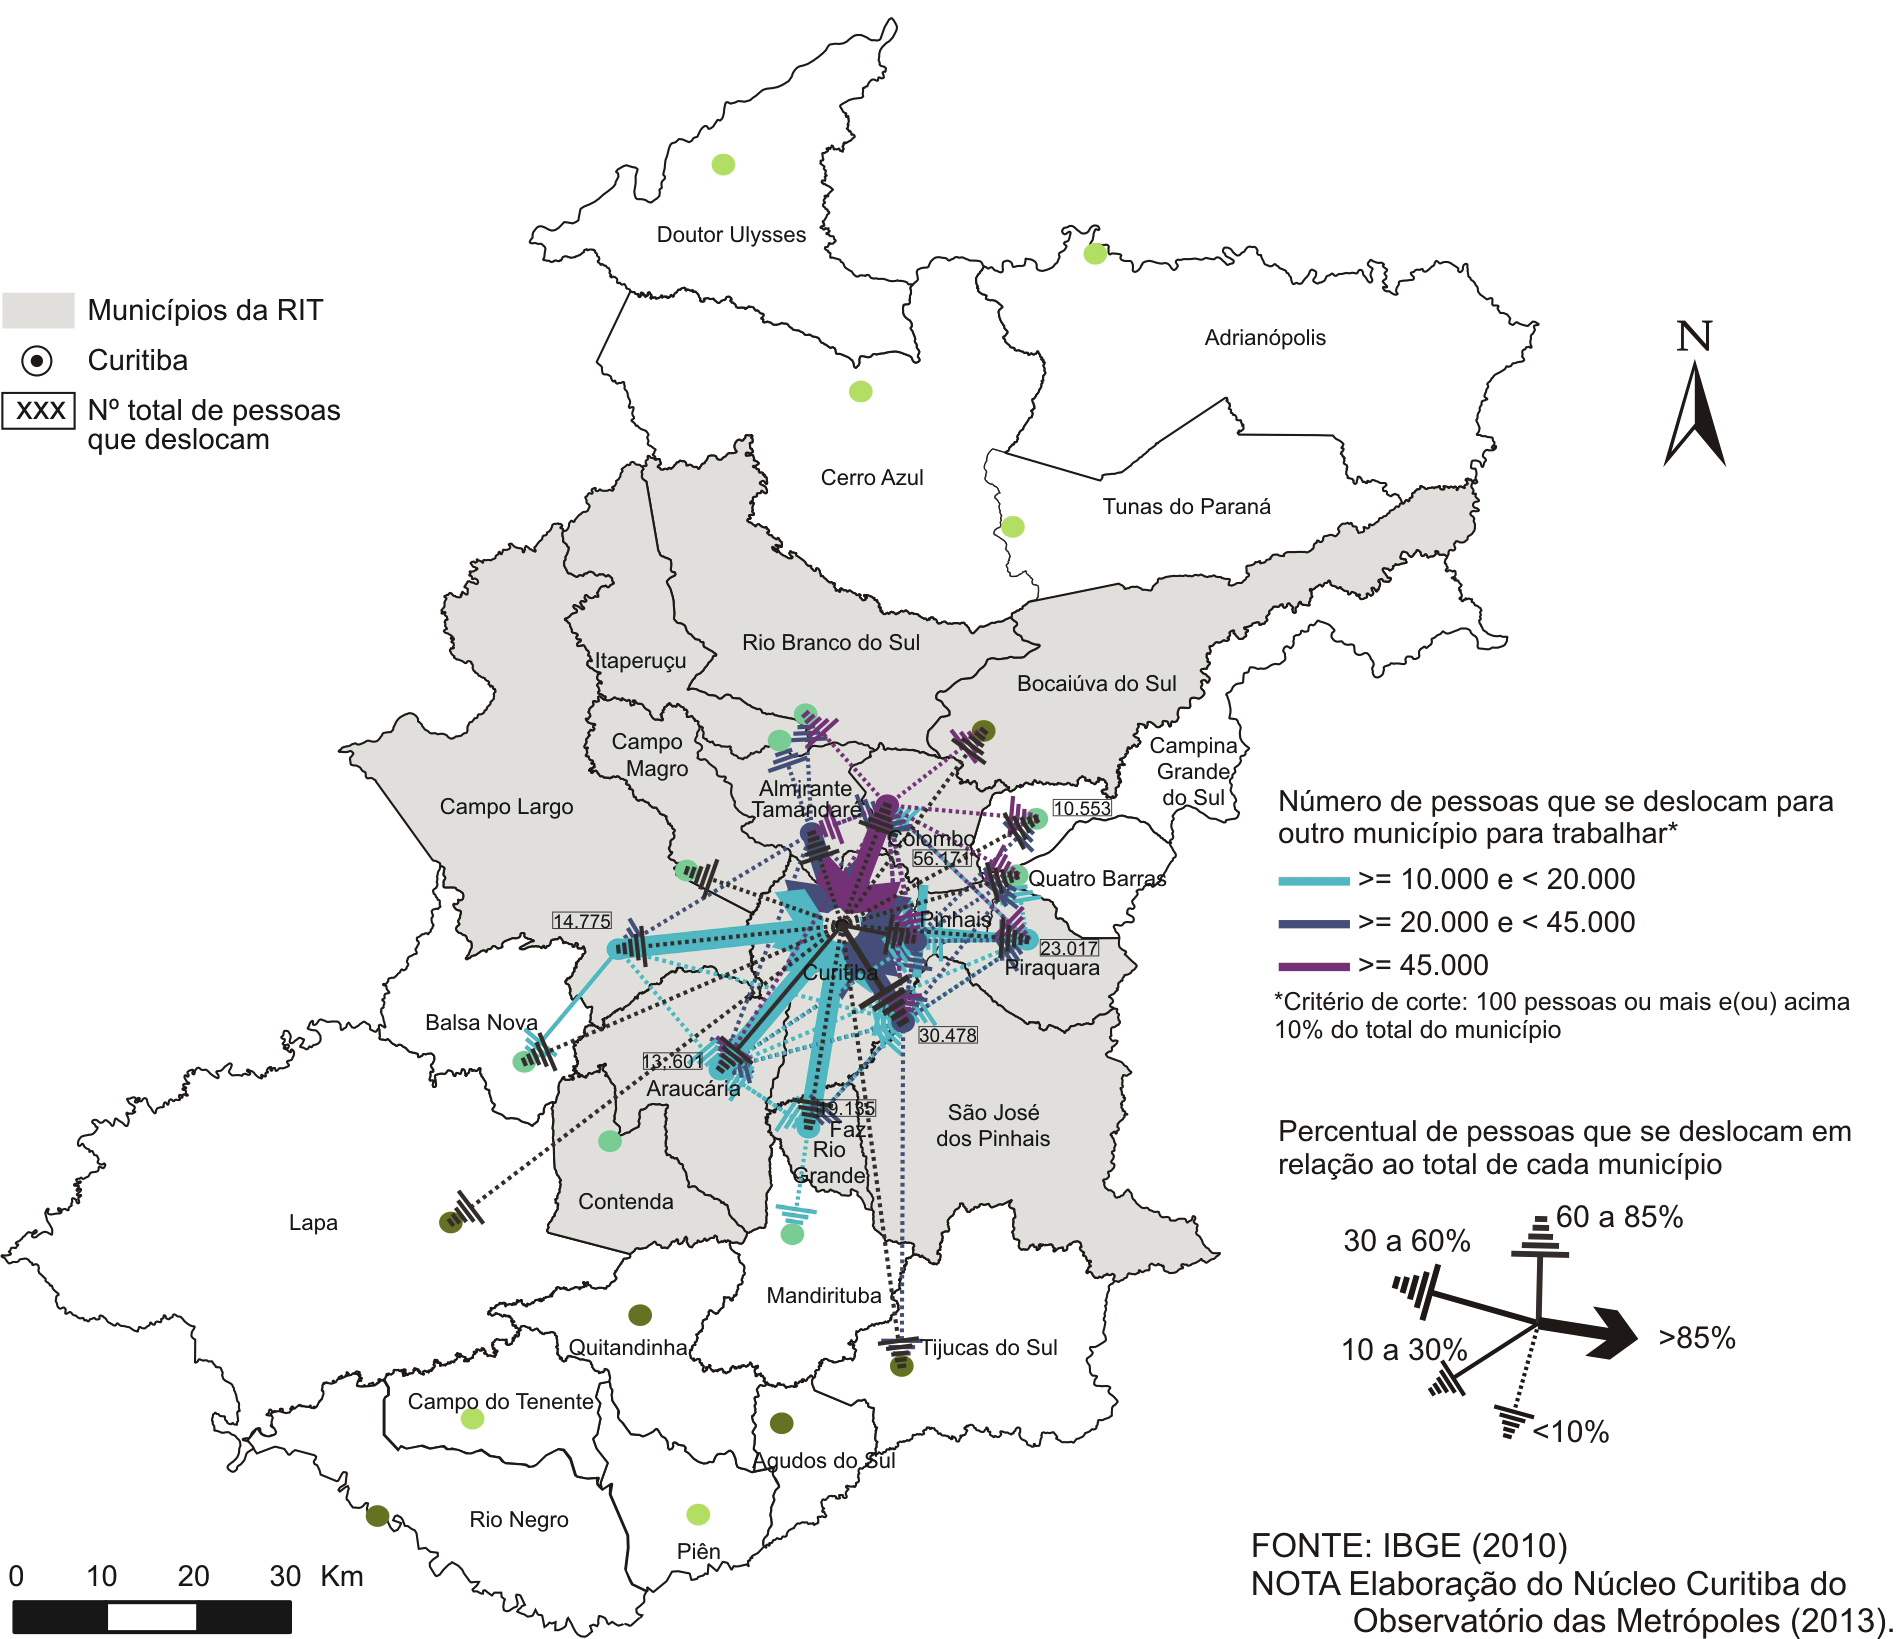
\includegraphics[width=0.7\linewidth]{img/paese2014a_01}
		\label{fig:paese2014a01}
		\legend{Fonte: \citeonline[p. 384]{paese2014a}}
	\end{figure}

	Como pode ser observado na \autoref{fig:paese2014a02}, que representa cartograficamente fluxos pendulares entre municípios com viagens inferiores a 10 mil por motivo de trabalho, existem viagens pendulares entre municípios da RMC que não passam por Curitiba, ocorrendo em duas tramas conforme Firkowski, Paese e Nagamine (2014, p. 384-385):(i) “setor norte-leste (Almirante Tamandaré, Itaperuçu, Rio Branco do Sul, Colombo, Bocaiúva do Sul, Campina Grande do Sul e Quatro Barras); e (ii) ``setor leste-sul (Quatro Barras, Pinhais, Piraquara, São José dos Pinhais, Fazenda Rio Grande e Araucária)''.

	\begin{figure}
		\centering
		\caption{Fluxo de pessoas dos municípios cujo número total que se desloca para outro município é menor do que 10.000 - \gls{rmc} - 2010}
		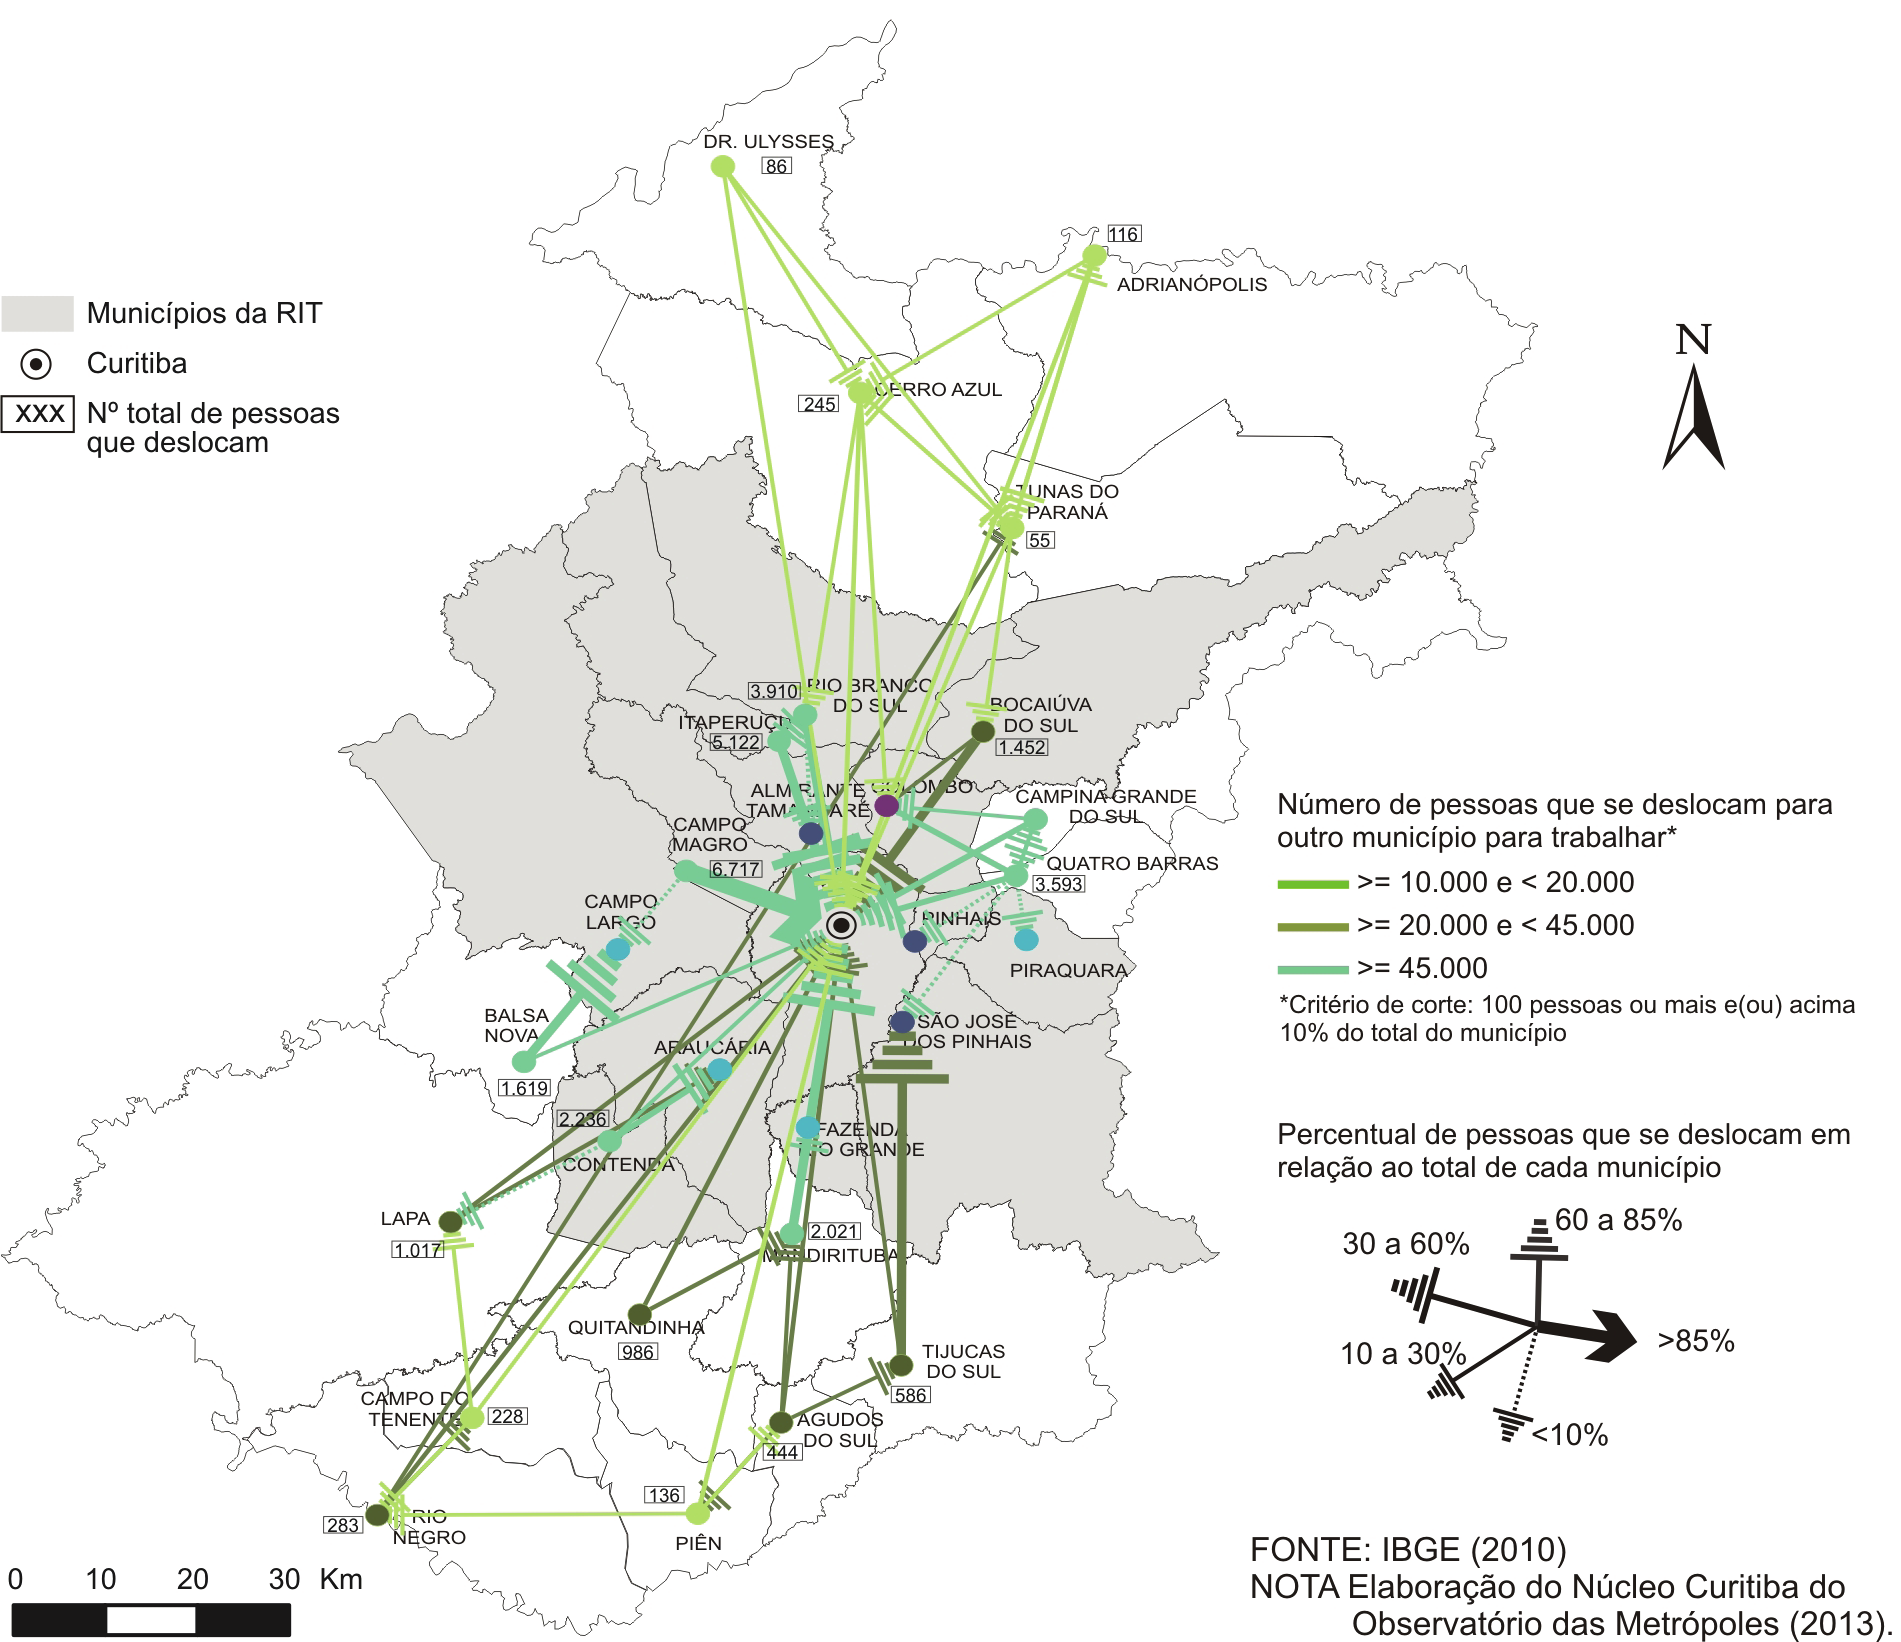
\includegraphics[width=0.7\linewidth]{img/paese2014a_02}
		\label{fig:paese2014a02}
		\legend{Fonte: \citeonline[p. 385]{paese2014a}}
	\end{figure}
	
	\section{Moradia como função pública de interesse comum}
	
	% fonte cadastrada como vaccari2018a no fontes.bib
	% plágio - p. 23 - https://acervodigital.ufpr.br/handle/1884/57167
	Utilizando-se do novo modelo de planejamento e gestão metropolitanos no estado do Paraná, exigência advinda da aprovação em 2015 da Lei Federal 13.089 - Estatuto da Metrópole -, é preciso compreender como os PDIs influenciam para a discussão da redefinição e gestão das FPICs na metrópole de Curitiba. Segundo o artigo que recebe o mesmo título deste subcapítulo, da autora Lorreini Vaccari, de acordo com os PDIs, verificou-se a interpretação da moradia como demanda metropolitana setorial, limitada à produção de habitação e lotes para a população de baixa renda, cabendo ao órgão metropolitano um papel auxiliar, de suporte à COPAHAR e à COHAB-CT. Observou-se também a não utilização de ferramentas e ações específicas e articuladas aos instrumentos de uso do solo para o tratamento da moradia na metrópole, confirmando-se que a questão não possui centralidade no planejamento metropolitano e nem é interpretada como FPIC geradora e articuladora das demais demandas urbano-metropolitanas. Segundo a autora, tal visão setorial é também recorrente e estruturante dos discursos, técnico e político vigentes. O não reconhecimento da moradia como FPIC contribui para o enfraquecimento do planejamento urbano na metrópole de Curitiba, bem como do próprio órgão metropolitano, que ao interpretar a moradia setorialmente e não articulada às demandas metropolitanas, limita sua ação e o potencial de seus efeitos sociais e territoriais, reproduzindo e contribuindo com o aprofundamento das desigualdades socioespaciais.
	
	A partir dessa perspectiva, e compreendendo a metrópole contemporânea como um produto do processo de metropolização do espaço, definido como um momento de maior complexidade da urbanização, é preciso que se articulem esses territórios urbanizados, que como demonstrado em seu desenvolvimento histórico, foi caracterizado pela fragmentação e aprofundamento das desigualdades socioespaciais e pela ampliação da polarização social, bem como pela complexificação das relações socioeconômicas e sociopolíticas.
	
	Historicamente, os planos e programas de investimento implementados pela COMEC não tiveram vigor suficiente para alterar a realidade do processo de produção do espaço metropolitano a partir da lógica de periferização e precarização da moradia que, capturada pela lógica de cidade mercadoria, produz uma metrópole cada vez mais marcada pela segregação socioespacial, permitindo evidenciar a moradia como questão fundamental e FPIC central para o planejamento metropolitano. 
	
	A questão da moradia também revela o modelo a partir do qual a metropolização brasileira tem se consolidado, com profundas desigualdades socioespaciais. Estudos realizados pela Fundação João Pinheiro em parceria com o Ministério das Cidades, apresentaram para o Censo de 2010, uma carência de 6 milhões e 940 mil unidades, com 85\% desse total localizado em áreas urbanas e déficit habitacional urbano relativo às regiões metropolitanas estimado em 3 milhões e 299 mil unidades, ou seja, aproximadamente 50\% do déficit habitacional do país (FJP, 2013).
	
	De acordo com a pesquisa de Vaccari, a constatação de que a moradia não foi arrolada legalmente como FPIC na RMC e não constitui elemento orientador da atuação da Coordenação da Região Metropolitana de Curitiba (COMEC), desde a sua criação, associada à atuação setorial e desvinculada de uma política pública de moradia metropolitana do Governo do Estado do Paraná e da Prefeitura Municipal de Curitiba no tratamento da problemática da moradia na metrópole, permitiram formular o problema de pesquisa, que parte basicamente do fato de que, se a moradia pode ser entendida como geradora das demais demandas da população urbano-metropolitana e, portanto, transversal e articuladora das demais FPICs, o não reconhecimento da moradia como questão central e crucial ao planejamento territorial, reforça o tratamento setorial das políticas urbanas, aprofundando as desigualdades socioespaciais. Assim, o não reconhecimento da moradia como FPIC pela entidade metropolitana contribui para o enfraquecimento do planejamento urbano como tributário do acesso à metrópole em Curitiba, bem como da própria entidade metropolitana, que deveria ser a instância mediadora e articuladora dos entes federativos para a gestão dos interesses comuns metropolitanos.
	
	\section{Outras funções públicas de interesse comum}
	
	A \gls{rmc} possui o Consórcio Intermunicipal para Gestão dos Resíduos Sólidos Urbanos, que é composto pelos municípios de: Almirante Tamandaré; Araucária; Balsa Nova; Campina Grande do Sul; Campo Largo; Campo Magro; Colombo; Contenda; Curitiba; Fazenda Rio Grande; Mandirituba; Pinhais; Quatro Barras; Quitandinha, e São José dos Pinhais. O prazo de duração do consórcio é indeterminado.
	
	\chapter{Gestão}
	
	\section{COMEC}
	
	\section{IPARDES}
	
	\section{IPPUC}
	
	\chapter{Orçamento e financiamento}
	
	Pendente. Ninguém contribuiu desde 14/out.
	
	\chapter{Governança}
	
	\chapter{Considerações finais}
	
	%===============================================================================
	%
	
	% ----------------------------------------------------------
	% ----------------------------------------------------------
	\postextual
	
	
	
	% informa o arquivo com a bibliografia. Deve ser o mesmo nome
	% (sem o sufixo) que será informado no ambiente filecontents
	% que está no final deste arquivo. Neste exemplo foi usado 
	% bibitemp.bib e bibtemp. Este comando insere a bibliografia
	% nesta posição (antes dos apêndices, anexos, índice remissivo)
	\bibliography{fontes}
	% ----------------------------------------------------------
	% Glossário
	% ----------------------------------------------------------
	% Consultar manual da classe abntex2 para orientações sobre o
	% uso do glossário.
	\renewcommand{\glossaryname}{Glossário}
	%\renewcommand{\glossarypreamble}{Esta é a descrição do glossário.\\ \\}
	\renewcommand*{\glsseeformat}[3][\seename]{\textit{#1}
		\glsseelist{#2}}
	
	% ---
	% Traduções para o ambiente glossaries
	% ---
	\providetranslation{Glossary}{Glossário}
	\providetranslation{Acronyms}{Siglas}
	\providetranslation{Notation (glossaries)}{Notação}
	\providetranslation{Description (glossaries)}{Descrição}
	\providetranslation{Symbol (glossaries)}{Símbolo}
	\providetranslation{Page List (glossaries)}{Lista de Páginas}
	\providetranslation{Symbols (glossaries)}{Símbolos}
	\providetranslation{Numbers (glossaries)}{Números} 
	% ---
	
	% ---
	% Imprime o glossário
	% ---
	\cleardoublepage
	\phantomsection
	\addcontentsline{toc}{chapter}{\glossaryname}
	% \glossarystyle{index}
	% \glossarystyle{altlisthypergroup}
	\glossarystyle{tree}
	\printglossaries
	% ---
	
	% ----------------------------------------------------------
	% Apêndices
	% ----------------------------------------------------------
	
	% ---
	% Inicia os apêndices. Não esquecer de fechar ao final de
	% todos os apêndices (\end{apendicesenv})
	% ---
	%\begin{apendicesenv}
	
	% Imprime uma página indicando o início dos apêndices
	%\partapendices
	
	% ----------------------------------------------------------
	%\chapter{Primeiro apêndice}
	% ----------------------------------------------------------
	
	%Este é um exemplo de inclusão de capítulos de %apêndice em uma 
	%monografia.  Cada apêndice é tratado como se fosse %um capítulo.
	%Os apêndices devem ser iniciados pelo comando de %ambiente
	%\textbackslash begin\{apendicesenv\} e encerrados %pelo comando 
	%\textbackslash end\{apendicesenv\}.
	
	% ----------------------------------------------------------
	%\chapter{Segundo apêndice}
	% ----------------------------------------------------------
	
	%Este é um exemplo de inclusão de um segundo apêndice. 
	
	%\end{apendicesenv}
	% ---
	
	
	% ----------------------------------------------------------
	% Anexos
	% ----------------------------------------------------------
	
	% ---
	% Inicia os anexos
	% ---
	%\begin{anexosenv}
	
	% Imprime uma página indicando o início dos anexos
	%\partanexos
	
	% ---
	%\chapter{Anexo I}
	% ---
	%Os anexos são similares aos apêndices se distinguindo pelo fato
	%que os apêndices são de autoria do autor da monografia e os 
	%anexos não são da autoria do autor da monografia.  Por exemplo,
	%se incluir no trabalho um modelo de um formulário preenchido
	%por alunos participantes de uma pesquisa, este será um apêndice
	%se o formulário foi criado pelo autor da monografia e será um
	%anexo se o formulário tiver sido criado por outros (por exemplo,
	%é um formulário padrão da escola em que o aluno que o preenche
	%estuda).
	%
	%Mesmo que o formulário tenha sido elaborado pela escola, uma
	%reprodução do formulário preenchido por cada aluno na pesquisa
	%será incluído no apêndice pois envolve o trabalho do autor da
	%monografia ao distribuir, coletar e reproduzir as respostas.
	%
	%Este é um exemplo de inclusão de capítulos de anexos em uma 
	%monografia.  Cada anexo é tratado como se fosse um capítulo.
	%Os anexos devem ser iniciados pelo comando de ambiente
	%\textbackslash begin\{anexoenv\} e encerrados pelo comando 
	%\textbackslash end\{anexoenv\}.
	%
	%\end{anexosenv}
	% ---
	%---------------------------------------------------------------------
	%---------------------------------------------------------------------
	
	%\printindex
	
	% Por padrão são incluídas no trabalho somente as referências
	% citadas ao longo do texto. No comando abaixo foram acrescentadas
	% algumas referências não citadas (neste texto servem apenas como
	% exemplos). Não deve ser usado o comando (mais simples) 
	% \nocite{*}, pois este parece não ser compatível com o
	% abntex2cite
	%\nocite{abntex2cite,abntex2wiki,boyer,eves,iezzi,kletenic,
	%        diomara,steinbruch,intusolatex,feynman,shannon,
	%        luisfelipe,turing}
\end{document}
